%% 美赛模板:正文部分

\documentclass[12pt]{article}  % 官方要求字号不小于 12 号,此处选择 12 号字体

% 本模板不需要填写年份,以当前电脑时间自动生成
% 请在以下的方括号中填写队伍控制号
\usepackage[2332102]{easymcm}  % 载入 EasyMCM 模板文件
\problem{Y}  % 请在此处填写题号
%\usepackage{mathptmx}  % 这是 Times 字体,中规中矩 
%\usepackage{mathpazo}  % 这是 COMAP 官方杂志采用的更好看的 Palatino 字体,可替代以上的 mathptmx 宏包
\usepackage{newtxtext}
\newcommand{\upcite}[1]{\textsuperscript{\textsuperscript{\cite{#1}}}} 
\title{Pricing Used Sailboats : A Combination Model Based on Heuristic Multilevel Regression and Deep Forest}  % 标题

% 如需要修改题头(默认为 MCM/ICM),请使用以下命令(此处修改为 MCM)
\renewcommand{\contest}{MCM}

% 文档开始
\begin{document}

% 此处填写摘要内容
\begin{abstract}
    Sailboats fulfill diverse roles, fueling a thriving second-hand market. 
    Brokers, facing numerous complex factors, struggle to determine reasonable pricing. 
    A tool is urgently needed to assist in comprehensive evaluations and rational pricing for used boats.

    This paper aims to construct a reliable model based on existing datasets, 
    which can provide a reasonable explanation for the pricing of the used sailboat market. 
    It also analyzes the impact of different factors and indicators on prices. 
    Finally, the model will be applied to the used sailboat market in Hong Kong to provide a reasonable and accurate pricing rule.

    For Data Exploration, we first try to preprocess the data with \textbf{Adaptive Density-Based Clustering} and \textbf{Linear Interpolation} methods.
    Moreover, we use the web strapper to fetch more data to expand the dimensions of our data. Simple statistical analysis shows that sub-indicators center around the \emph{year}, \emph{variant}, and \emph{region}.
    
    For Problem(a), Inspired by the previous conclusion, we adopt a \textbf{Heuristic Multilevel Regression Model} for making the three \emph{discrete} variables \emph{continuous}, introduce the concept of \textbf{impurity} to heuristically evaluate interrelation among variables, and avoid bias by introducing \textbf{feedback and renormalization}. Finally, we use \textbf{Deep Forest} to regress them to the price.
    And our model achieves good precision on both the train set and the test set.

    For Problem(b), 
    We apply \textbf{statistic analysis} of the distribution of the average price to find the regions' impacts.
    After using \textbf{normalization techniques} and \textbf{impurity analysis}, it can be concluded that the regional effect is not significant across variants and primarily takes effect by featuring variants of different prices.
    Practically and statistically, the GDP per capita is found of a linear correlation with the average variant prices of a region with \textbf{linear correlation coefficient} and \textbf{p-testing}.

    For Problem(c),
    our model can be fitted into the Hong Kong market using our model's \textbf{regional sub-indicators}.
    Besides, we spot a significant underestimation of our model when fitting it into Hong Kong's market in the subset of the catamarans' market.
    however, this regional effect is not found in the subset of the monohulled sailboats market. 
    
    For Problem(d), we find interesting patterns between the length and the region.

    Finally, we conducted an analysis of the strengths and weaknesses of our model. Besides, we further \textbf{optimized the model} and the results demonstrate that our model exhibits high levels of robustness, precision, and accuracy. After that, a report is attached.




    % 美赛论文中无需注明关键字。若您一定要使用,
    % 请将以下两行的注释号 '%' 去除,以使其生效
    \vspace{5pt}
    \textbf{Keywords}: Used Sailboat Pricing, Adaptive Density-Based Clustering, Heuristic Hierarchical Multiple Regression, Feedback Model, Deep Forest Model, Analysis of Variance.
 

\end{abstract}

\maketitle  % 生成 Summary Sheet
\tableofcontents  % 生成目录


% 正文开始
\section{Introduction}
% 问题背景
\subsection{Background}
In our daily lives, sailboats are not only a means of transportation but also serve as leisure, entertainment, and even for competitive sports. As a result, the growing demand for sailboats has given rise to a thriving boat market, which has developed into a second-hand market. In the market, buyers and sellers usually trade through brokers, who play a crucial role in the transaction process.

For brokers, it is essential to be familiar with the second-hand sailboat market, comprehensively consider various factors, and make reasonable pricing for the used sailboats in order to facilitate a successful transaction. However, the factors affecting the price of used sailboats are numerous and complex, with different brands, variants of boats, years, depreciation rates, as well as local consumption levels and geographical environments having significant impacts. The intertwined influences of these complex factors make it difficult to determine the pricing in the used sailboat market, and it is challenging to come up with a reasonable price that takes all factors into account.

Therefore, brokers urgently need a tool to assist them in making more reasonable and comprehensive evaluations of used sailboats and to make the pricing in the used sailboat market more rational.
%问题重述
\subsection{Problem Restatement}
\textbf{Problem (a) :}
\begin{itemize}
    \item Develop a prediction model to explain the listing price of each of the sailboats in the provided spreadsheet.
    \item Discuss the precision of our estimate for each sailboat variant's price.
\end{itemize}

\textbf{Problem (b) :}
\begin{itemize}
    \item Determine whether Region has an impact on the price of second-hand boats and explain the effect.
    \item Discuss whether any regional effect is consistent across all sailboat variants.
    \item Address the practical and statistical significance of any regional effects noted.
\end{itemize}

\textbf{Problem (c) :}
\begin{itemize}
    \item Based on the model, find out how it can be useful in the Hong Kong market.
    \item Choose one subset and model the regional effect of Hong Kong on each sailboat's prices.
    \item Assess whether the effect is the same for both catamarans and monohull sailboats.
\end{itemize}

\textbf{Problem (d) :}
\begin{itemize}
    \item Identify and discuss additional informative conclusions drawn from the data.
\end{itemize}

\textbf{Problem (e) :}
\begin{itemize}
    \item Create a one-to-two-page report with well-chosen graphics to help the Hong Kong sailboat broker to understand your findings.
\end{itemize}
%我们的工作
\subsection{Our work \& Model Overview}
\begin{figure}[htbp]
    \centering
    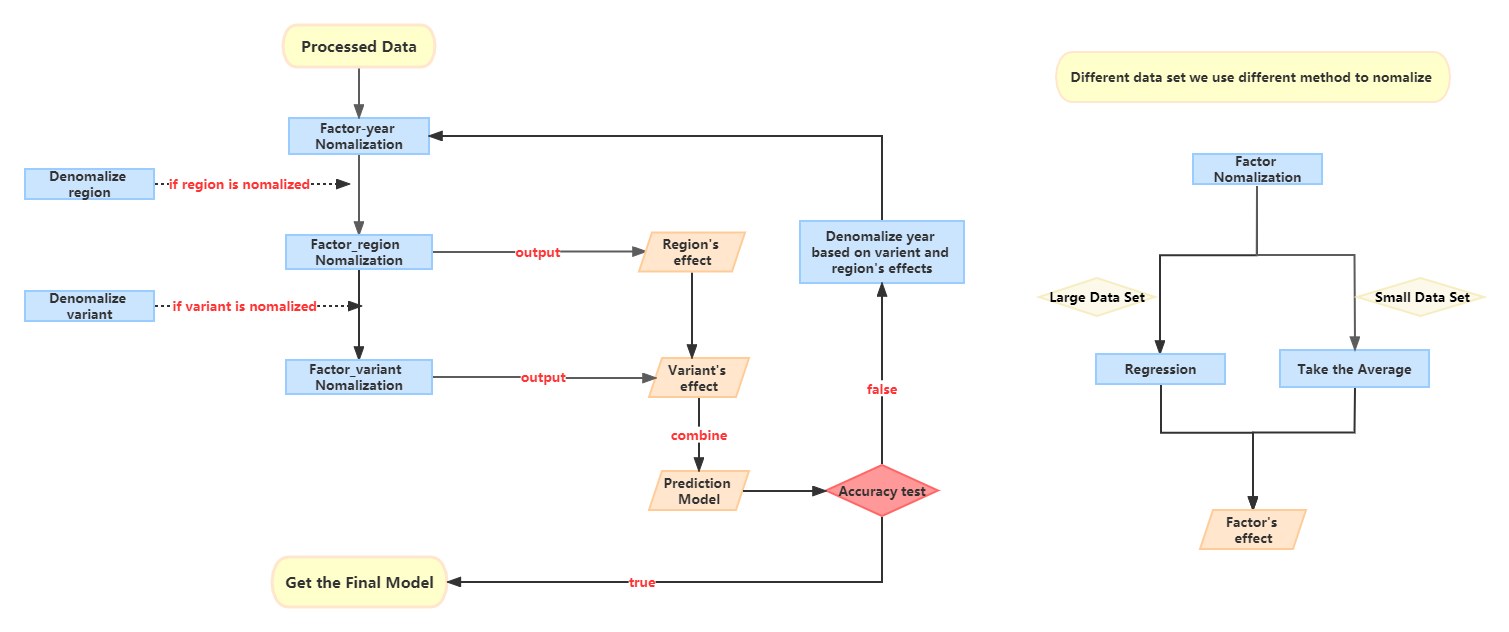
\includegraphics[width=1\textwidth]{OurWork.png}
    \caption{Model Framework}\label{fig:OurWork}
\end{figure}
Our team began by meticulously cleaning, expanding, and pre-analyzing the dataset using \textbf{Adaptive Density-Based Clustering} and \textbf{Linear interpolation} techniques. These methods allowed us to identify patterns and trends in the data, preparing it for subsequent modeling.

Then, we utilized a \textbf{Hierarchical Multiple Regression} to abstractly express the Region's Effect and Variant's Effect, to achieve the continuous representation of the two discrete variables, Region and Variant. Next, we applied \textbf{Linear Regression} to obtain the relationship between Year, Region Effect, Variant Effect, and Price. This approach helped us capture the interactions between these variables and their influence on the pricing.

Following this, we employed a \textbf{Deep Forest Model} to estimate the relationship between region and variant indicators and their respective effects. This advanced ensemble learning technique allowed us to predict the effect of unknown regions and variants, which in turn enabled us to further predict their prices.

As a result, we successfully developed a comprehensive and robust model (Figure \ref{fig:OurWork}) that is well-suited for Hong Kong brokers when pricing used sailboats. By leveraging the strengths of both Heuristic Hierarchical Multiple Regression and Deep Forest Models, our approach offers a reliable and accurate way to estimate the value of sailboats based on indicators in the dataset. This model serves as a valuable tool for brokers and other stakeholders in the sailboat market, facilitating informed decision-making and ensuring fair pricing practices.

\section{Assumptions and Justifications}
% 问题假设
\subsection{Assumptions}
To simplify our problems, we make the following basic assumptions, each of which is
adequately justified.
\begin{itemize}
    \item The price of used sailboats is solely determined by the factors in the dataset.
    \item The factors in the dataset are independent and unrelated.
    \item The data in the dataset are all real, reasonable, and follow a certain pattern.
    \item For the used boats that need price prediction, we can obtain at least the same number of factors information as in the dataset.
    \item The pricing required by a broker should be reasonable and in accordance with market rules, rather than false pricing.
\end{itemize}
%符号含义
\subsection{Notations}
\ 
% 三线表示例
\begin{table}[!htbp]
\begin{center}
\begin{tabular}{cc}
	\toprule

	Symbol& Definition\\
	\midrule
	$l$ &Measurement data\\
    \hline
	$L$ &Feature vector\\
    \hline
	$F$ &The dimension of $L$\\
    \hline
    $k$ &Search range\\
    \hline
    $\lambda$ & The feature values of natural neighbors\\
    \hline
    $nb_k(l)$ & The number of reverse neighbors of $l$ in the $k$-th iteration\\
    \hline
    $R$ & Correlation coefficient\\
    \hline
    $\hat{y}$ & The estimated value of $y$\\
    \hline
    $\hat{\beta}$ & The estimated value of the regression coefficients\\
    \hline
    $P$ & Measured value \\
    \hline
    $Q$ & Simulated value \\ 
    \hline
    $\alpha$ & p-value significance level \\
    \hline
    $df$ & freedom \\
    \hline
    $s$ & standard deviation \\
    \hline 
    $T$ & t-distribution \\

	\bottomrule
\end{tabular}
\end{center}
\end{table}

\section{Data Exploration}

\begin{figure}[htbp]
    \centering
    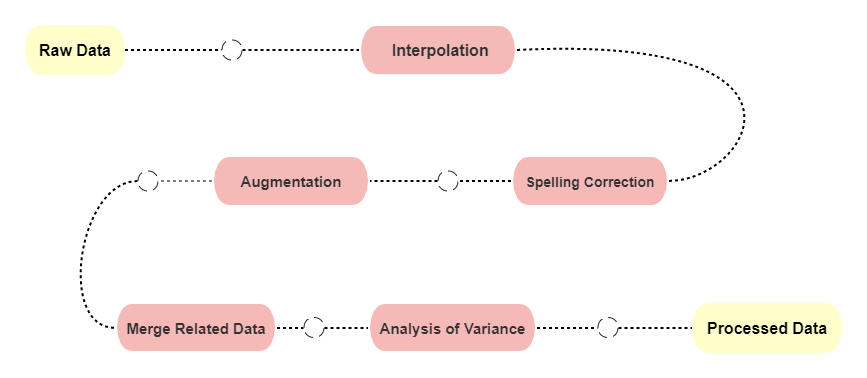
\includegraphics[width=.8\textwidth]{Data.png}
    \caption{Data Exploration}\label{fig:Data}
\end{figure}

\subsection{Data Cleaning}
First of all, we turn the given \textbf{\texttt{xlsx}} format data sheet into \textbf{\texttt{csv}} format. 
The conversion causes some minor errors like extra spaces and unexcepted characters which can be easily filtered out by text editor and python string operating functions like \textbf{\texttt{strip()}} or so.

Secondly, we use \textbf{Linear interpolation} to fill in the missing data and then apply \textbf{Adaptive Density-Based Clustering} for spell correction,
resulting in a more complete and accurate dataset than the original.

Specificlly:

Based on the text-type variables, the feature matrix $L_i$ is used, and the Euclidean distance is used to calculate the text similarity:
$$dist(l_i,l_j)=\sqrt{\sum_{f=1}^{F}(L_i^f-L_j^f)^2}$$

Because ADC is a clustering iterative process, we first calculate the $k$-Nearest Neighbors:
$$NN_k(l_i)=\{l_j \in D|dist(l_i,l_j)\leq dist(l_i,o)\}$$

Then we define the Reverse Neighbors as:
$$RNN(l_i)=\{l_j \in D|l_i\in NN_k(l_j)\}$$

Applying $NN_k$ and $RNN(l)$ iteratively to obtain clustering centers, unclassified text samples are assigned to the nearest clustering center, and $\lambda$ is calculated as follows:
$$\lambda=\min\{k|\sum_{i=1}^{n}f(nb_k(l_i))=0\quad or\quad \sum_{i=0}^{n}f(nb_k(l_i))=\sum_{i=0}^{n}f(nb_{k-1}(l_i))\}$$

Where $f(x)$ is defined as:
$$f(x)=
\begin{cases}
0,\quad otherwise\\1,\quad if\quad x=0
\end{cases}$$

Further more, we merge \textbf{Make} into \textbf{Variant} into a single feature, which we refer to as \textbf{Variant}.

Finally, we merge the corrected dataset with the accurate one after making necessary modifications.
\begin{figure}[htbp]
    \centering
    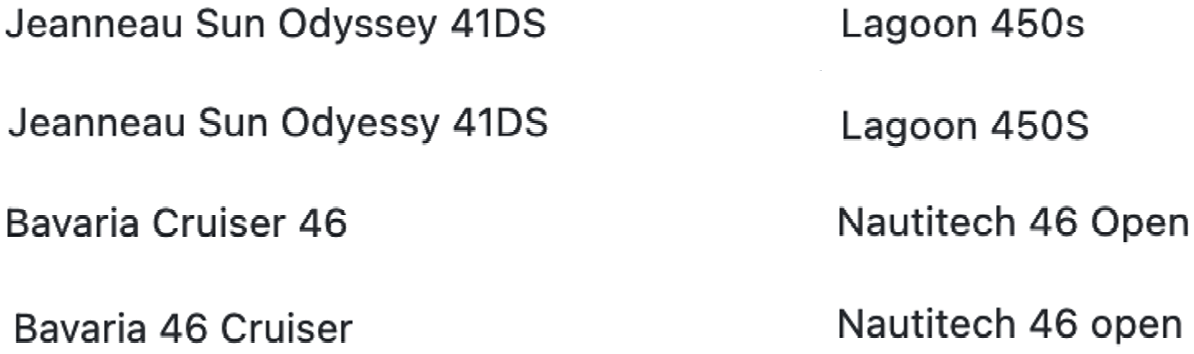
\includegraphics[width=0.7\textwidth]{error_data.png}
    \caption{Examples of error data}\label{fig:error_data}
\end{figure}

\subsection{Data Augmentation}

Our team diligently collected and organized additional ship attributes for the given dataset using Pandas' \texttt{read\_html} web scraping technique,
which allowed us to efficiently extract valuable information from various online sources. 
Simultaneously, we gathered the 2020 GDP per capita  data of the relevant regions to provide important economic context that might influence sailboat prices.

Upon obtaining the data, we first employed Pandas' related functions to remove any duplicate entries, 
ensuring the dataset's integrity and uniqueness. 
Next, we addressed missing values by using linear interpolation, 
a technique that estimates missing data points by drawing upon the values of neighboring data points. 
This approach helped us create a more complete and reliable dataset for further analysis.

These data collection, organization, and preprocessing efforts significantly enriched the diversity of the data and expanded the dataset dimension.
By incorporating a wider range of sailboat features and relevant economic data, we were able to develop a more comprehensive understanding of the factors influencing sailboat prices. 
This extensive dataset laid a solid foundation for our subsequent modeling efforts, enabling us to create more accurate and reliable predictive models for sailboat pricing.





\subsection{Data Analysis}
There is a lot of labels related to sailboat specifications, which is complicated and may have mutually subtle relationship.
Therefore, it is challenging to discuss their individual influence on listing prices.
Attempting to directly perform regression on these labels using machine learning models can lead to \textbf{overfitting issues}, where the model becomes too specialized in fitting the training data and loses its ability to generalize well to new, unseen data.

Despite these challenges, we can still extract some relatively straightforward insights from the data, which can provide valuable theoretical support for our subsequent modeling efforts:
\begin{itemize}
    \item Time: Time is a quasi-continuous and ordered variable, exhibiting a clear linear relationship with the price of sailboats (as demonstrated in Figure \ref{fig:year_price} and Table \ref{table: correlation_coefficient}). As sailboats age, their value typically decreases, reflecting factors such as depreciation, wear and tear, and technological advancements in newer models.
    \item Variant and Region: These factors are undeniably related to sailboat prices; however, their unordered and non-continuous nature necessitates further analysis. Sailboat variants can encompass different designs, sizes, and features, which can significantly impact their value. Similarly, regional factors such as local demand, availability, economic conditions, and even cultural preferences can influence sailboat prices.
\end{itemize}
\begin{figure}[htbp]
    \centering
    \begin{subfigure}[b]{.4\textwidth}
    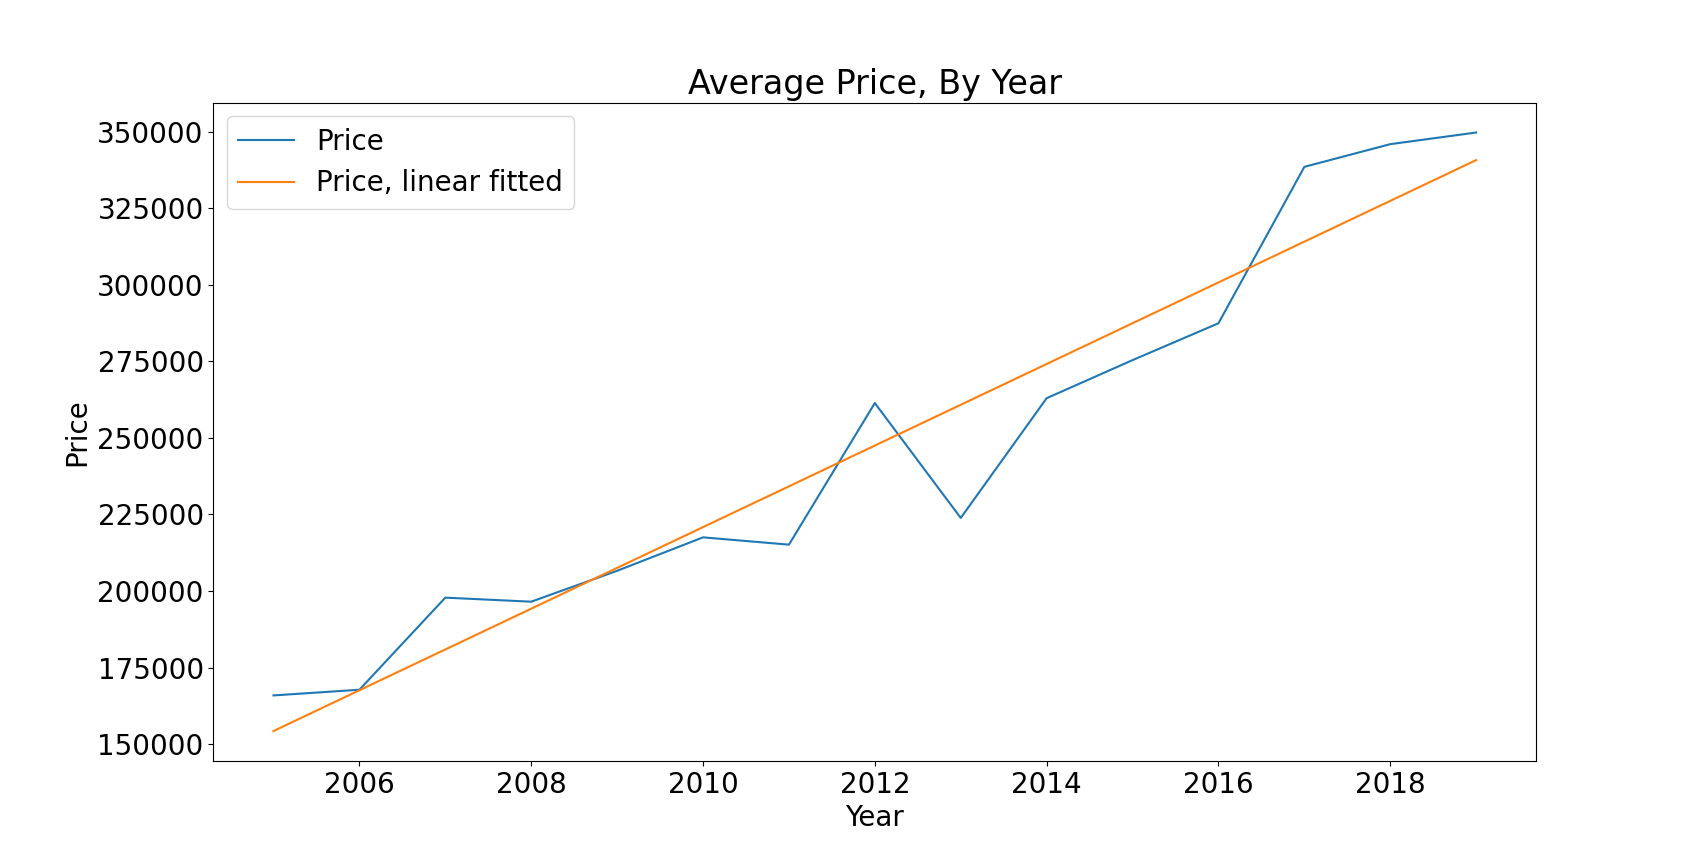
\includegraphics[width=\textwidth]{monohulled_price_year.png}
    \caption{Monohulled Sailboats}\label{subfig:mono_year}
    \end{subfigure}
    \begin{subfigure}[b]{.4\textwidth}
    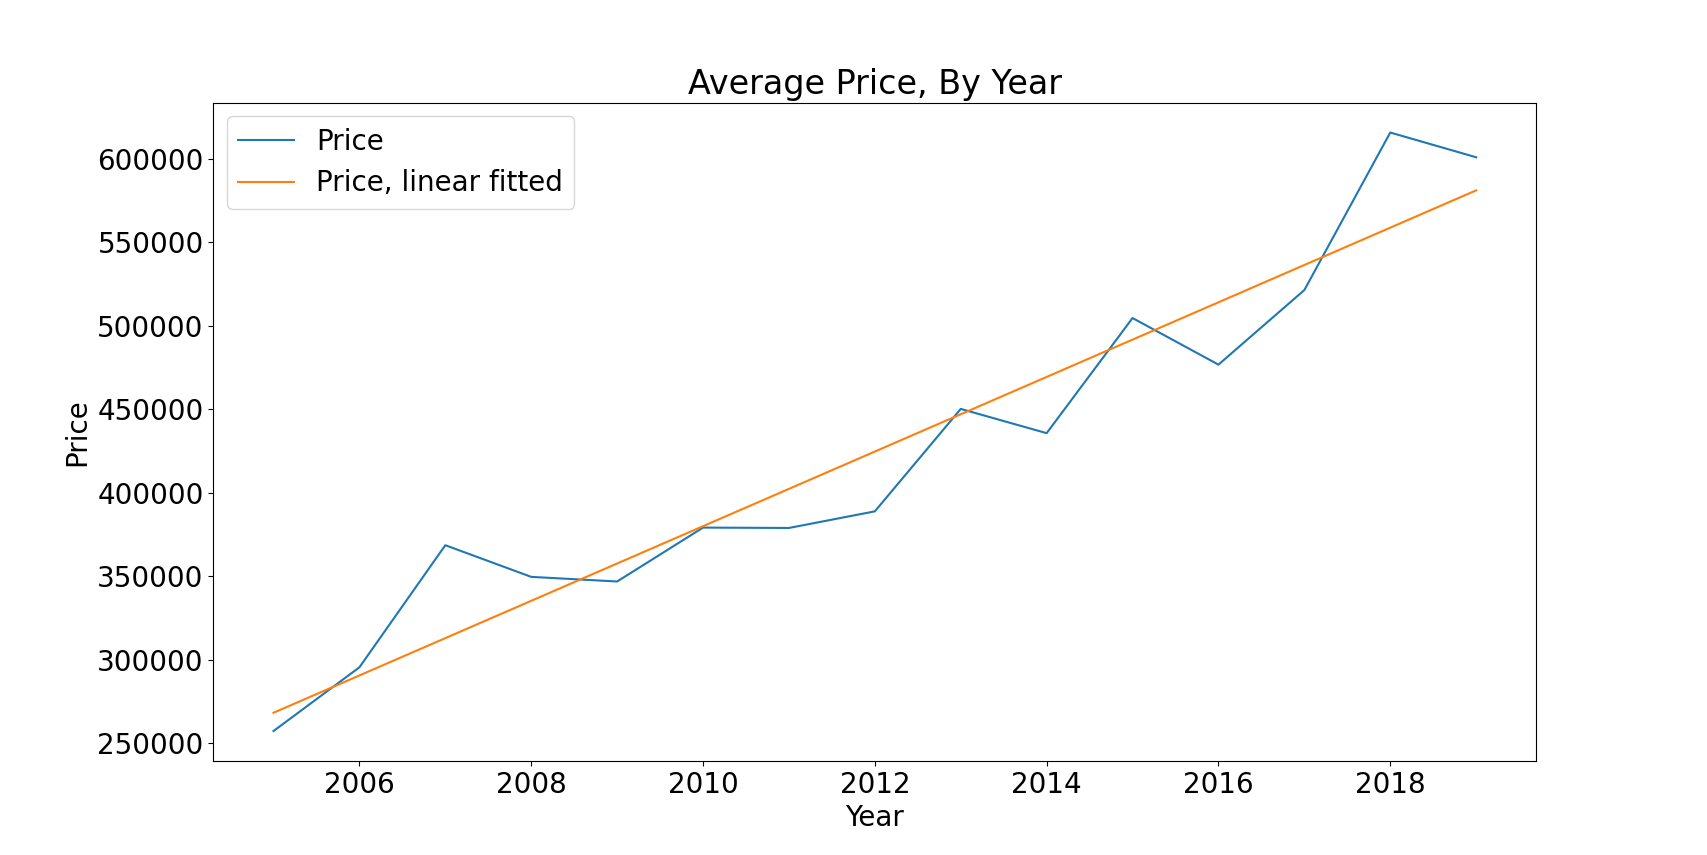
\includegraphics[width=\textwidth]{catamaran_price_year.png}
    \caption{Catamaran}\label{subfig:cata_year}
    \end{subfigure}
    \caption{The relationship between year and price}\label{fig:year_price}
\end{figure} 

\begin{table}[h!]
    \begin{center}
      \begin{tabular}{c|c|c|c}
        & Pearson & Spearman & Kendall\\
        \hline
        \hline
        Monohulled Sailboats&0.964 & 0.989 & 0.943 \\
        Catamaran  &0.960& 0.971 & 0.867\\
      \end{tabular}
      \caption{The correlation coefficient of year and price}\label{table: correlation_coefficient}
    \end{center}
\end{table}


\section{The Prediction Model of Used Sailboat Prices}

\subsection{The Establishment of The Model}
\subsubsection{Model 1 \textemdash  Heuristic Hierarchical Multiple Regression}
Inspired by the conclusion drawn from data analysis, we adopt a multilevel heuristic model that utilizes the purity of the samples grouped by specific variables.  We introduce impurity to model a variable's independence from other variables.

To be specific, we begin with the year variable mentioned above.

The impurity by a variable can be measured by the weighted mean variance of all groups divided by the variable.

Unavoidably, the initial impurity will damage our model's accuracy. For example, we have supposed that the year variable is independent of other variables for the first round of normalization (otherwise we cannot resolve the problem at the beginning), making our normalizing coefficient of this variable biased.

Therefore, we introduce the feedback model into our model. To be exact,   after the first round has been completed, compared to the initial state, we have more information about the year, variant, and region factors' effect. Therefore, we repeatedly renormalize the factors to gain a more accurate coefficient (factors' effect).

Specifically, \emph{Model 1}, as illustrated in Figure \ref{fig:Model1}, is specifically designed to predict prices by taking into account input variables such as Year, Region, and Variant. To achieve accurate predictions, this model incorporates a heuristic hierarchical multiple regression approach, which distinguishes it from conventional regression methods. This innovative technique allows for a more nuanced understanding of the relationships between variables, ultimately leading to improved performance and reliability.

As for Hierarchical Multiple Regression, to solve the objective function for a given $n$ data points $(x_i, y_i)$:
$$L(y,f(x,w))=\sum_{i=1}^{n}[y_i-f(x_i,w_i)]^2$$

To get the coefficient matrix, we typically use the least squares method to solve it:
$$\min f(x)=\sum_{i=1}^{n}L^2_i(x)=\sum_{i=1}^{n}L_i^2[y_i,f(x_i,w_i)]=\sum_{i=1}^{n}[y_i-f(x_i,w_i)]^2$$

The matrix is illustrated as:
$$\hat{\beta}=(X^TX)^{-1}X^TY=(\sum x_ix_i^T)^{-1}(\sum x_iy_i)$$

Then we get the predicted value:
$$\hat{y} = \hat{\beta_0} + \hat{\beta_1} x_1 + \hat{\beta_2} x_2 + ... + \hat{\beta_p} x_p$$

In the hierarchical multiple regression process, each layer focuses on one variable, denormalizing it while normalizing the other two variables. The price generated at this stage is regarded as the Effect of the specific variable under consideration. Simultaneously, the fitting result from the current layer is used as the baseline for normalization in the next layer, which is then incorporated into the regression. This iterative process continues until the model achieves a precise fitting effect, ensuring optimal performance and an accurate understanding of the relationships between variables.
\begin{figure}[htbp]
    \centering
    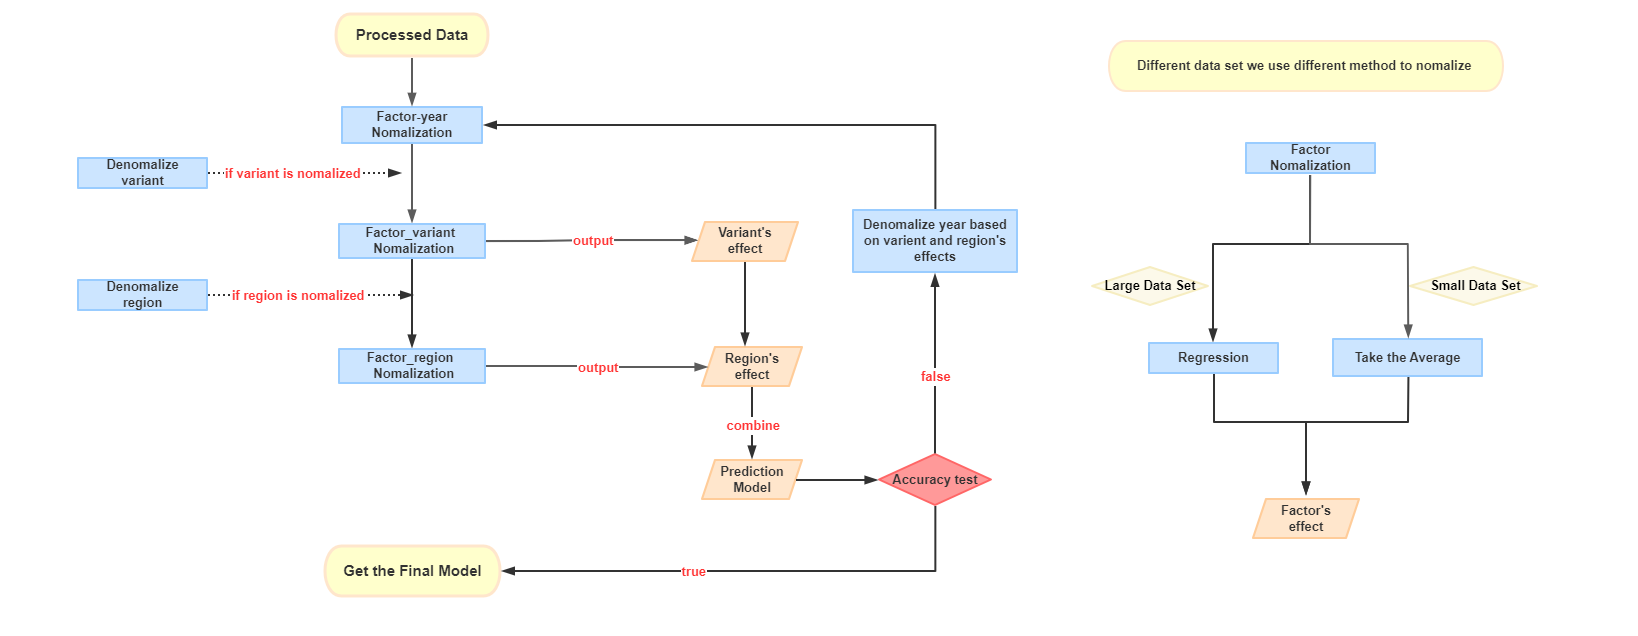
\includegraphics[width=1\textwidth]{Model1.png}
    \caption{Brief process of Model 1}\label{fig:Model1}
\end{figure}
A key aspect of \emph{Model 1}'s success is the heuristic approach employed during each normalization step. This method adapts to the size of the dataset, offering a more efficient and effective means of processing the data. For larger datasets, regression is performed, which capitalizes on the wealth of information available and can identify complex patterns and relationships. Conversely, for smaller datasets, the model calculates the average, providing a simpler and more straightforward representation of the data.

\begin{figure}[htbp]
    \centering
    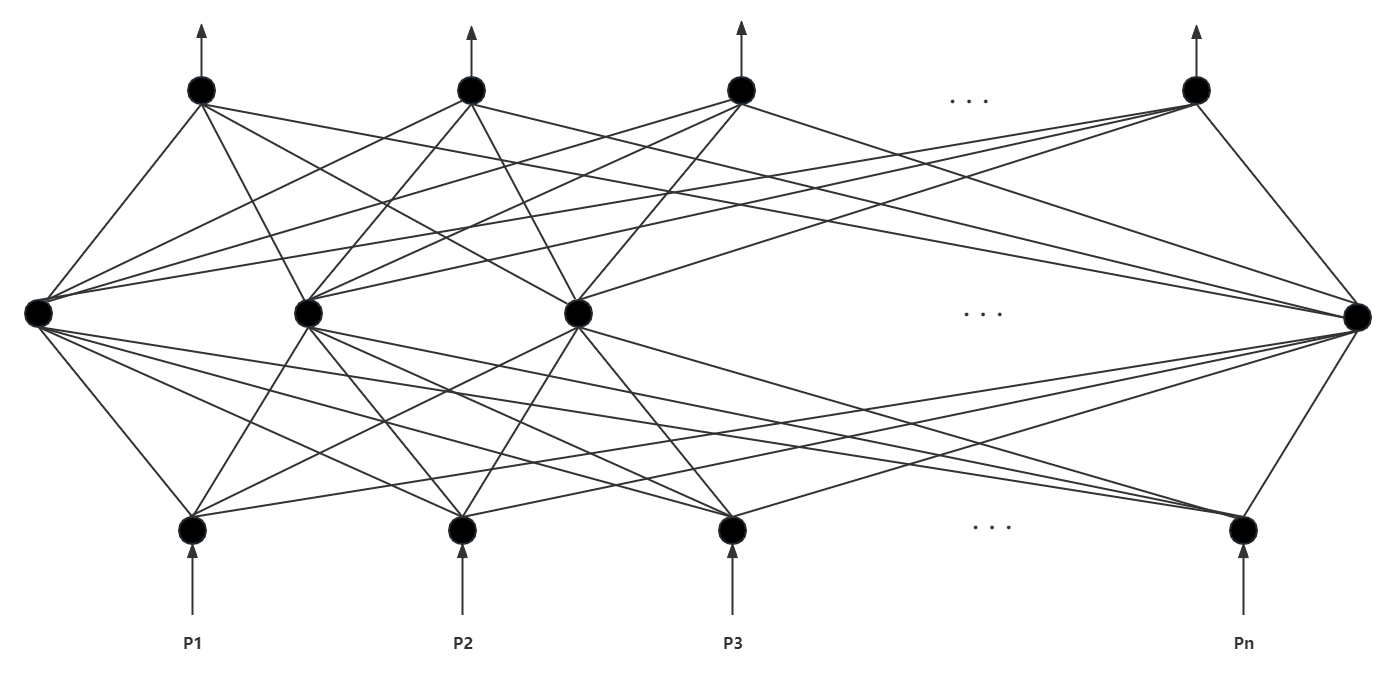
\includegraphics[width=.6\textwidth]{Hierarchical.png}
    \caption{Hierarchical Multiple Regression}\label{fig:Hierarchical}
\end{figure}

This adaptive heuristic approach has a significant impact on the accuracy of the model's predictions, as it tailors the normalization process to suit the specific characteristics of the dataset. By adjusting the method used based on dataset size, \emph{Model 1} is better able to understand the underlying patterns and relationships, leading to more accurate and reliable predictions.


\subsubsection{Model 2 \textemdash  Deep Forest Model}


However, the regression prediction based on \emph{Model 1} is incomplete, as \emph{Model 1} requires the variant and region of the data being predicted to have appeared in the dataset before. In practice, the variant and region might be unseen by the Model. For instance, in the third question, \emph{Model 1} cannot predict the prices in Hong Kong since the Model has not assessed the region's effect for Hong Kong. Therefore, we employed the Deep Forest algorithm to establish \emph{Model 2}.

\begin{figure}[htbp]
    \centering
    \includegraphics[width=1\textwidth]{Deep_forest1.png}
    \caption{Deep Forest Model}\label{fig:DF1}
\end{figure}

Decision trees are a common machine learning method, with both classification and regression models. Initially, we used a basic decision tree for regression, but the model had a large error and poor accuracy for predicting prices. As a result, we optimized the model using the Deep Forest algorithm. Deep Forest is an ensemble learning model based on random forests. Unlike traditional decision trees, Deep Forest uses randomized strategies to train each tree-based classifier, increasing the model's diversity. Compared to a single decision tree, the Deep Forest model is more robust. The simplified process is as follows:

\begin{figure}[htbp]
    \centering
    \includegraphics[width=.8\textwidth]{Deep_forest2.png}
    \caption{Deep Forest Model}\label{fig:DF2}
\end{figure}


First, we expanded the dataset to obtain quantitative data for the region and variant. Specifically, for the variant, we expanded data such as draft, beam, water tank, fuel tank, cabins, and displacement. For the region, we expanded data such as GDP per capita, Gini coefficient, and Human Development Index. When dealing with unmarked variants and regions, we first applied \emph{Model 1} to obtain the effect of marked variants and regions. Then, we applied the effect of marked variants and regions to the Deep Forest, regressing through the expanded data to obtain the effect of unmarked variants and regions, and thus predicting the price.

\begin{figure}[htbp]
    \centering
    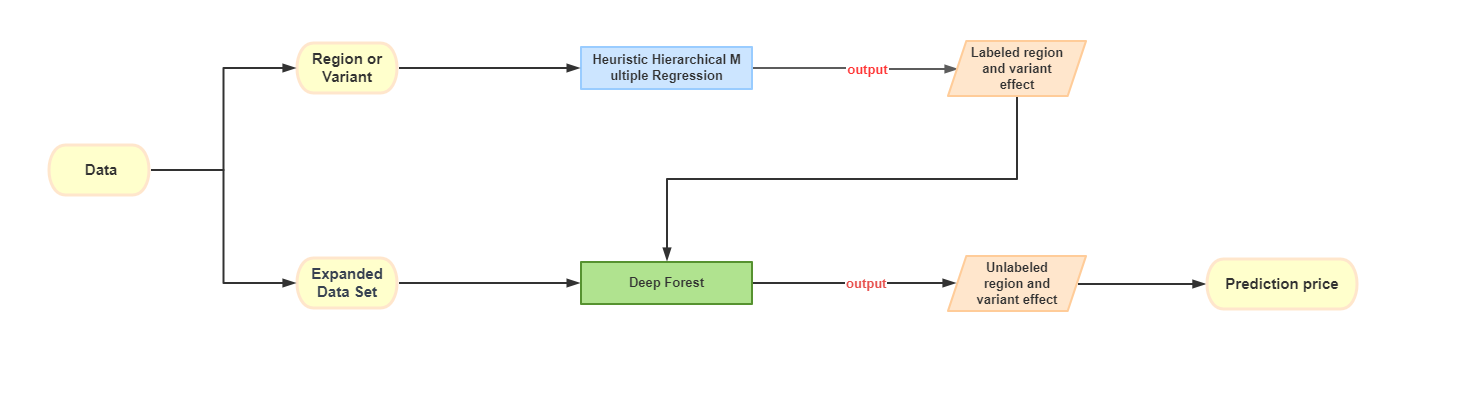
\includegraphics[width=1\textwidth]{Model2.png}
    \caption{Brief process of Model 2}\label{fig:Model2}
\end{figure}


\subsection{Model Accuracy Analysis}
Due to the limited data provided for some sailship types, 
they belong to imbalanced datasets. 
Therefore, we need to use as much data as possible for training to prevent the loss of small-sample data during training. 
Given that the leave-one-out method is not affected by random partition, 
it is effective for small-sample and imbalanced datasets, 
and can accurately evaluate the performance of the model, 
we used the \textbf{leave-one-out method} to analyze the model's error in the error analysis part.
  
For accuracy analysis, we use the correlation coefficient $R$ and Mean Absolute Percentage Error (MAPE) as evaluation metrics.
$$R(\textbf{X},\textbf{Y})=\frac{\text{cov}(\textbf{X},\textbf{Y})}{\sqrt{\text{var}[\textbf{X}] \text{var}[\textbf{Y}]}}$$
$$\text{MAPE} = \frac{\sum_{i = 1}^n (\frac{|\textbf{P} - \textbf{Q}|}{\textbf{P}} \times 100\%)}{n}$$
where:
    $$\text{var}(\textbf{X})=\frac{\sum_{i=1}^{n}(\textbf{X}_i-\overline{\textbf{X}})(\textbf{X}_i-\overline{\textbf{X}})}{n-1}$$
    $$\text{cov}(\textbf{X},\textbf{Y})=\frac{\sum_{i=1}^{n}(\textbf{X}_i-\overline{\textbf{X}})(\textbf{Y}_i-\overline{\textbf{Y}})}{n-1}$$

    \begin{figure}[htbp]
        \centering
        \begin{subfigure}[b]{.4\textwidth}
        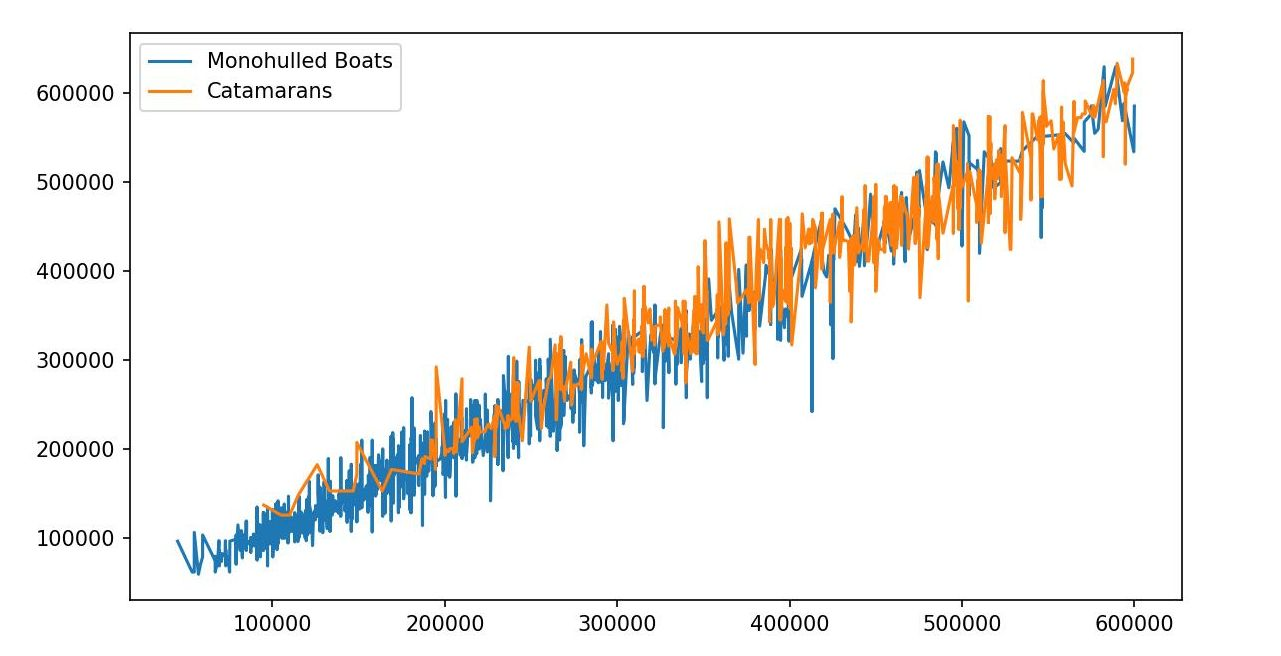
\includegraphics[width=\textwidth]{accuracy1.jpg}
        \caption{The fitting performance before denoising.}\label{subfig:accuracy1}
        \end{subfigure}
        \begin{subfigure}[b]{.4\textwidth}
        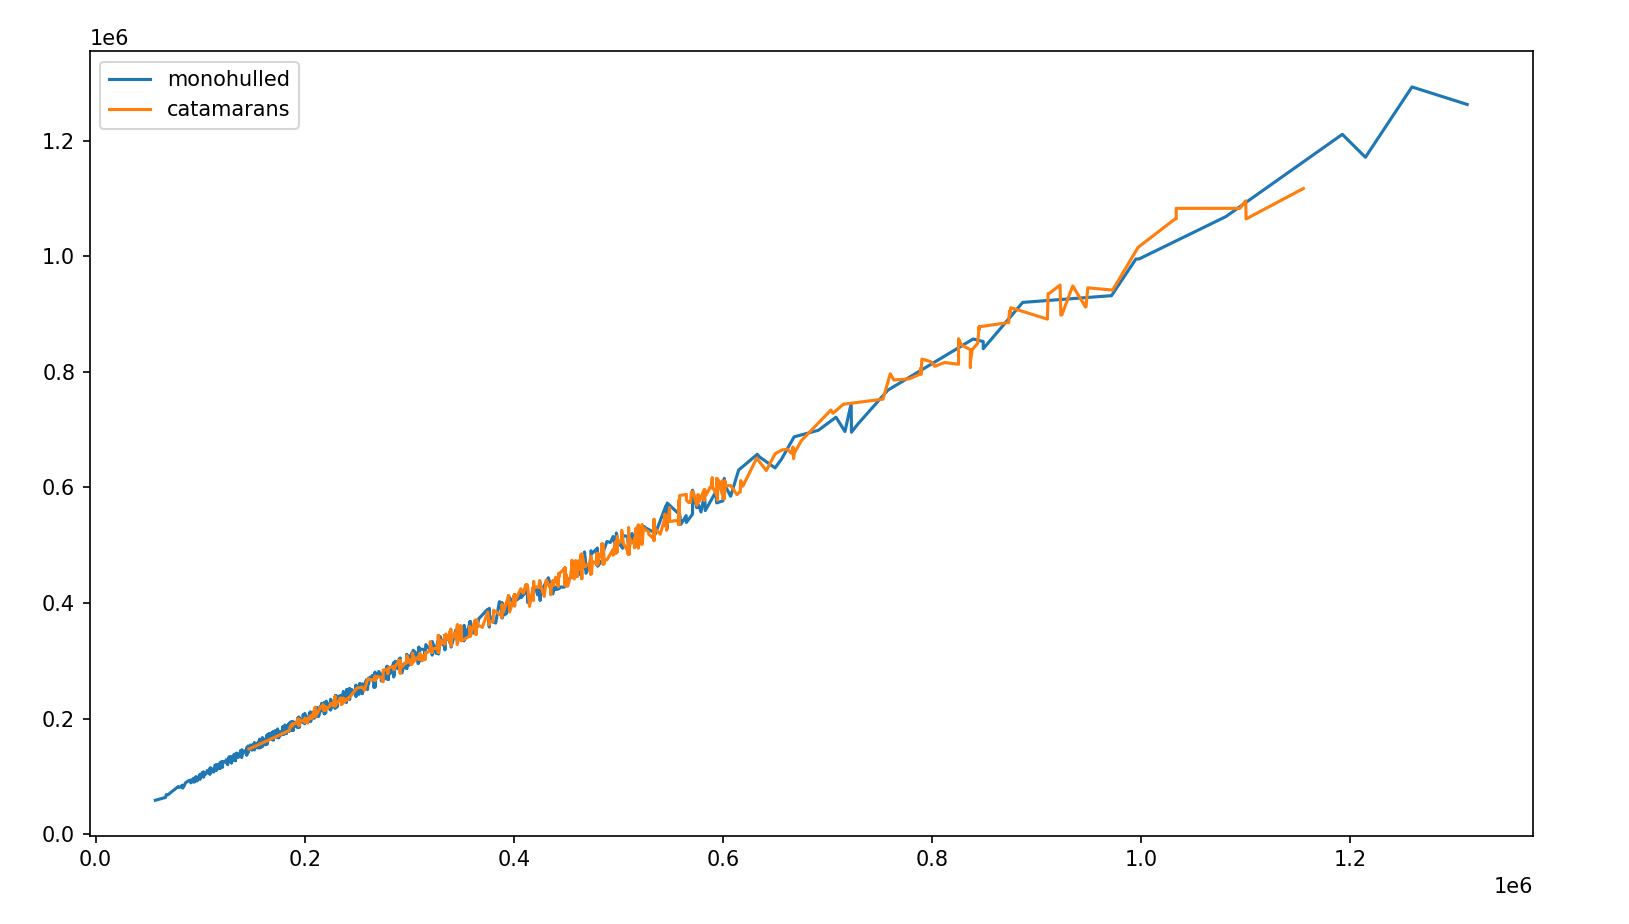
\includegraphics[width=\textwidth]{accuracy2.png}
        \caption{The fitting performance after denoising.}\label{subfig:accuracy2}
        \end{subfigure}
        \caption{Model Fitting Accuracy in HongKong}\label{fig:accuracy}
    \end{figure} 


\begin{table}[htbp]
        \centering
        \begin{tabular}{c|c|c}
        Train& Cata& Mono \\
        \hline
        \hline
        $R^2$ & 0.924 & 0.974 \\
        \hline
        MAPE & 5.09\% & 7.29\% \\
        \hline
        \end{tabular}
        \qquad
        \begin{tabular}{c|c|c}
        Test& Cata& Mono \\
        \hline
        \hline
        $R^2$ & 0.901 & 0.942 \\
        \hline
        MAPE & 10.16\% & 11.65\% \\
        \hline
        \end{tabular}
        \qquad
        \begin{tabular}{c|c|c}
        HK& Cata& Mono \\
            \hline
            \hline
            $R^2$ & 0.849 & 0.885 \\
            \hline
            MAPE & 7.18\% & 8.70\% \\
            \hline
            \end{tabular}
        \caption{Accuracy of Train Set, Test Set and HK Set}
        \label{tab:Accuracy}
\end{table}


\section{Regional Effect Analysis}

Applying \emph{Model 1}, we can easily abstract the effect of each region. 
Therefore, by normalizing the year and variant, 
we can clearly see the effect of each region(see Figure \ref{fig:region_effect1}).

\begin{figure}[htbp]
    \centering
    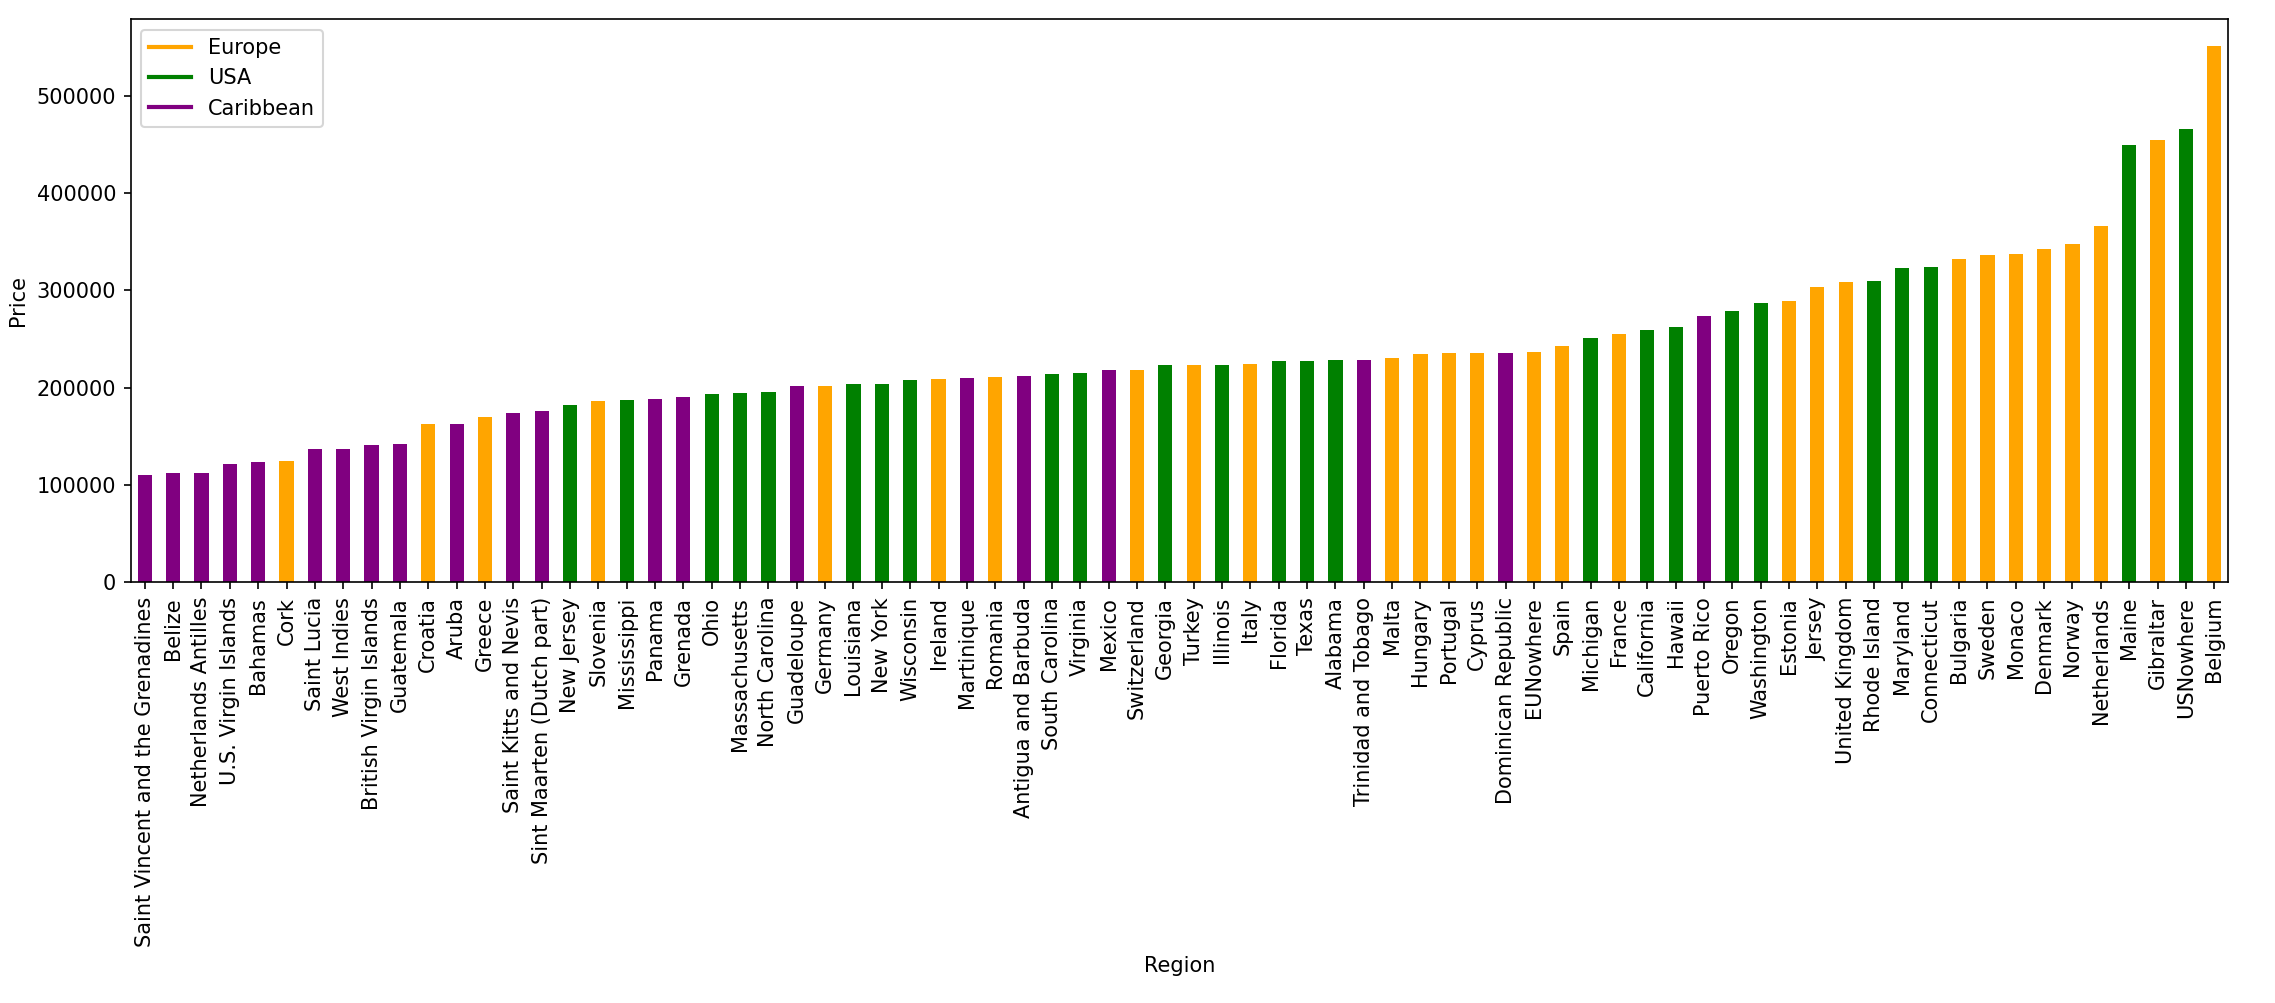
\includegraphics[width=1\textwidth]{region_effect1.png}
    \caption{Region's Effect}\label{fig:region_effect1}
\end{figure}

After normalizing the year and the variant factor (thus eliminating their influence), we surprisingly find that the distribution of average price among regions turns much more uniform than that of the initial state. Moreover, the imparity by variants is small as soon as the year factor is normalized(see Figure \ref{fig:region_effect2}). So we can conclude that the regional effect is not significant across variants. And it's necessary to note that the regional effect mainly takes effect by featuring variants of different prices.

Practically, the economic development level of the region best describes the region effect we found. Statistically, the GDP per capita is found of a strong positive linear correlation with the average variant prices of a region with linear correlation coefficient and p-testing.


\begin{figure}[htbp]
    \centering
    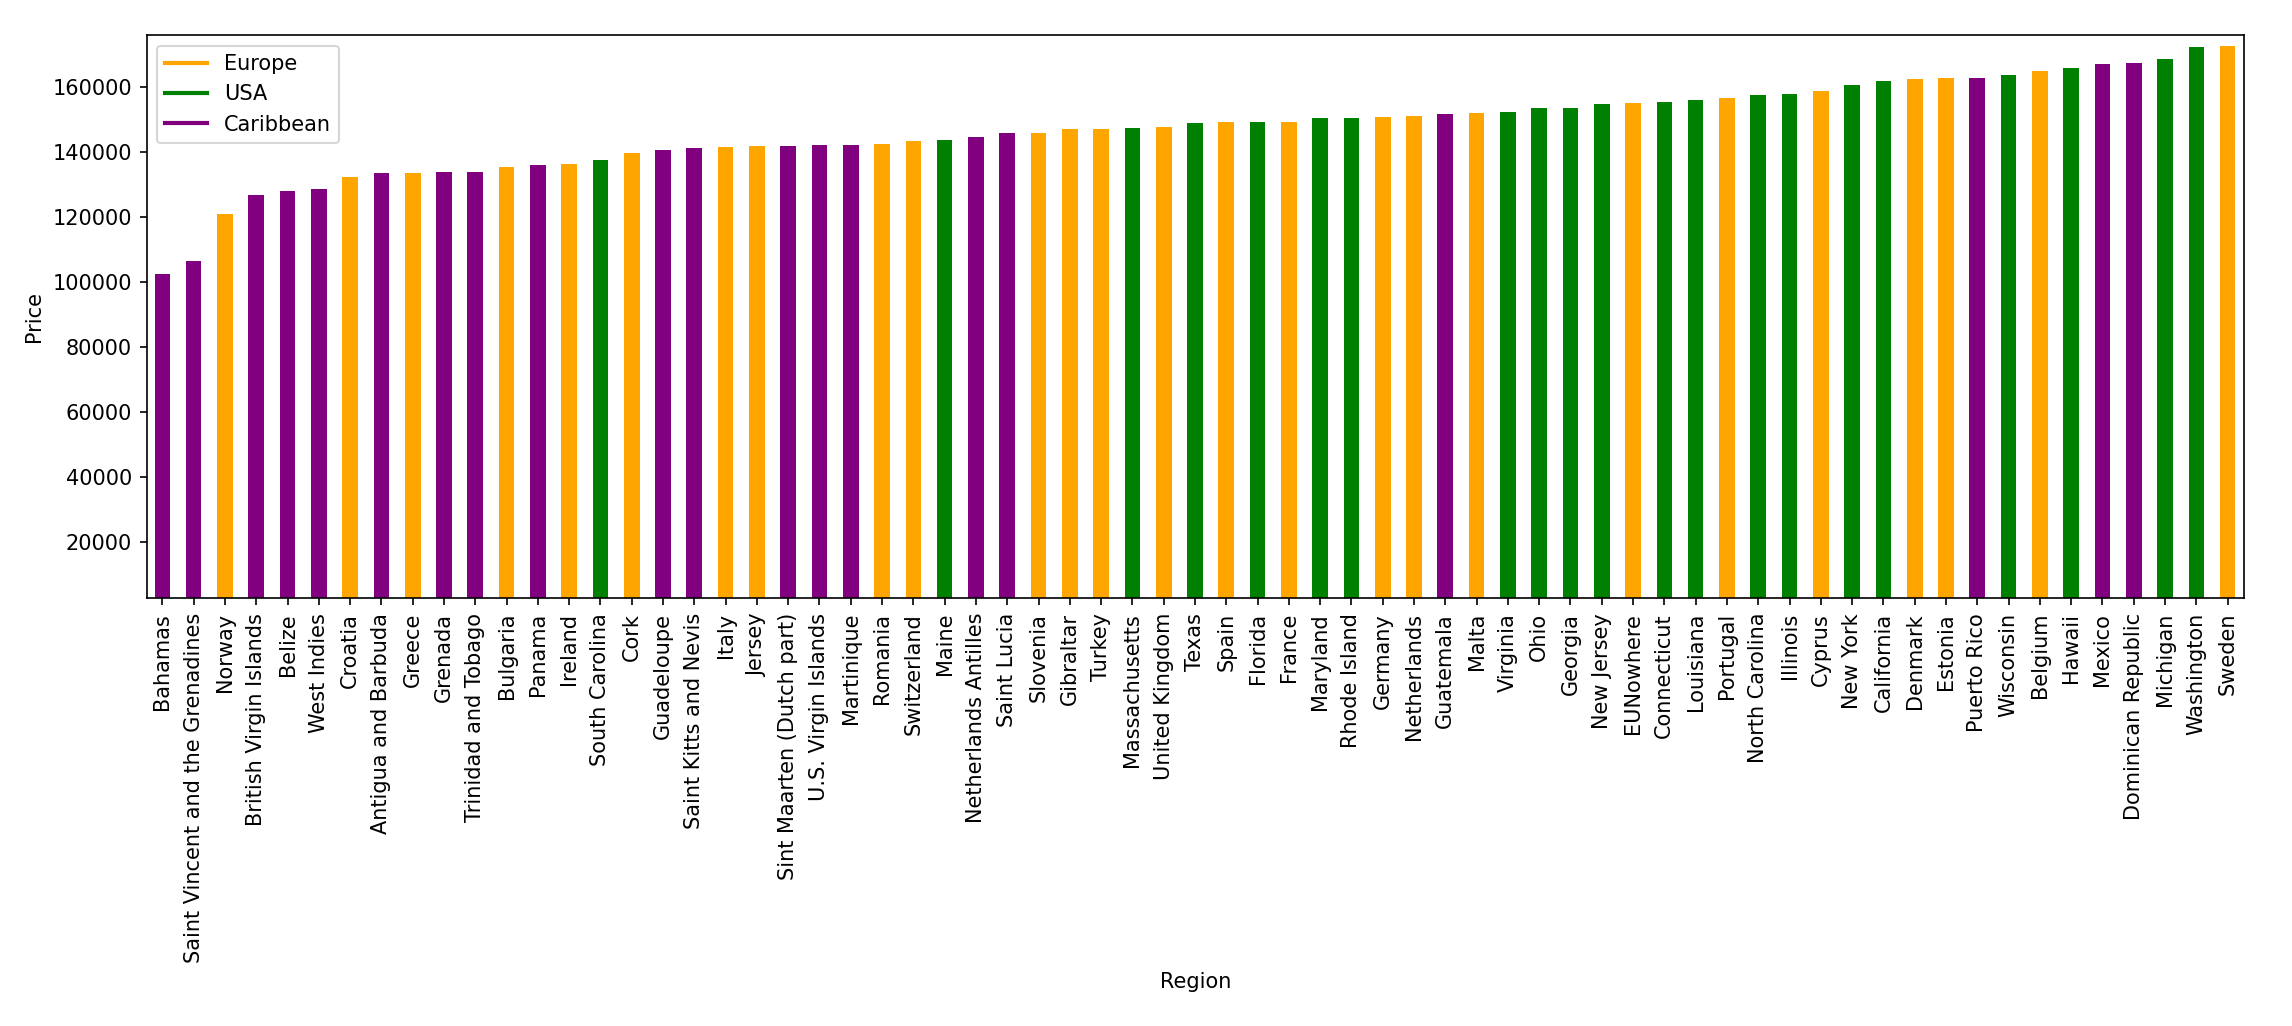
\includegraphics[width=0.9\textwidth]{region_effect2.png}
    \caption{Region's Effect after nomarlizing Variant}\label{fig:region_effect2}
\end{figure}

To verify the significance of linear correlation, we should perform p-testing:
Assuming that we choose $\alpha$ as the significance level for the p-value test (usually 0.01, 0.05, or 0.10) and the hypothesis is denoted as $H_0$, we first calculate the means and standard deviations of the two samples, denoted as $\bar{x}$ and $s$. Then, we calculate the t-value using the following formula:
$$t=\frac{\bar{x}_1-\bar{x}_2}{\sqrt{\frac{s_1^2}{n_1}+\frac{s_2^2}{n_2}}}$$

We calculate the degrees of freedom as $df = n_1 + n_2 - 2$, and then use the degrees of freedom and the significance level to look up the critical value of t from the t-distribution table with n-1 degrees of freedom. From this, we obtain the p-value:
$$p=2\times P(T>|t|)$$

Because we need to make a judgment about the correctness of the hypothesis $H_0$, we need to perform the following evaluation:
$$\begin{cases}
    p \geq\alpha ,\quad cannot \quad reject\quad H_0\\p<\alpha,\quad can \quad reject\quad H_0
    \end{cases}$$

\section{The Applicability of The Prediction Model in Hong Kong}
When applying our model to the Hong Kong region, 
we first try to obtain the indicators for the used sailboats. 
For Hong Kong, we start by using \emph{Model 2} to determine the Region's Effect, leveraging the area's GDP per capita data.

If the predicted Variant is present in the training set, 
we can directly use \emph{Model 1} to estimate the pricing by incorporating the Region's Effect, Variant's Effect, and Year. 
However, if the predicted Variant is not in the training set, we first need to use \emph{Model 2} to obtain the Variant's Effect by considering factors such as beam, draft, and displacement. 
Once the Variant's Effect is determined, we can then employ \emph{Model 1} to make the final price prediction.

This two-step approach enables us to adapt our models to different regions like Hong Kong and successfully predict used sailboat prices. 
By utilizing both \emph{Model 1} and \emph{Model 2} in tandem, we can account for regional influences, specific variant characteristics, 
and the age of the sailboat to provide accurate and reliable pricing estimates.

\begin{figure}[htbp]
    \centering
    \begin{subfigure}[b]{.4\textwidth}
    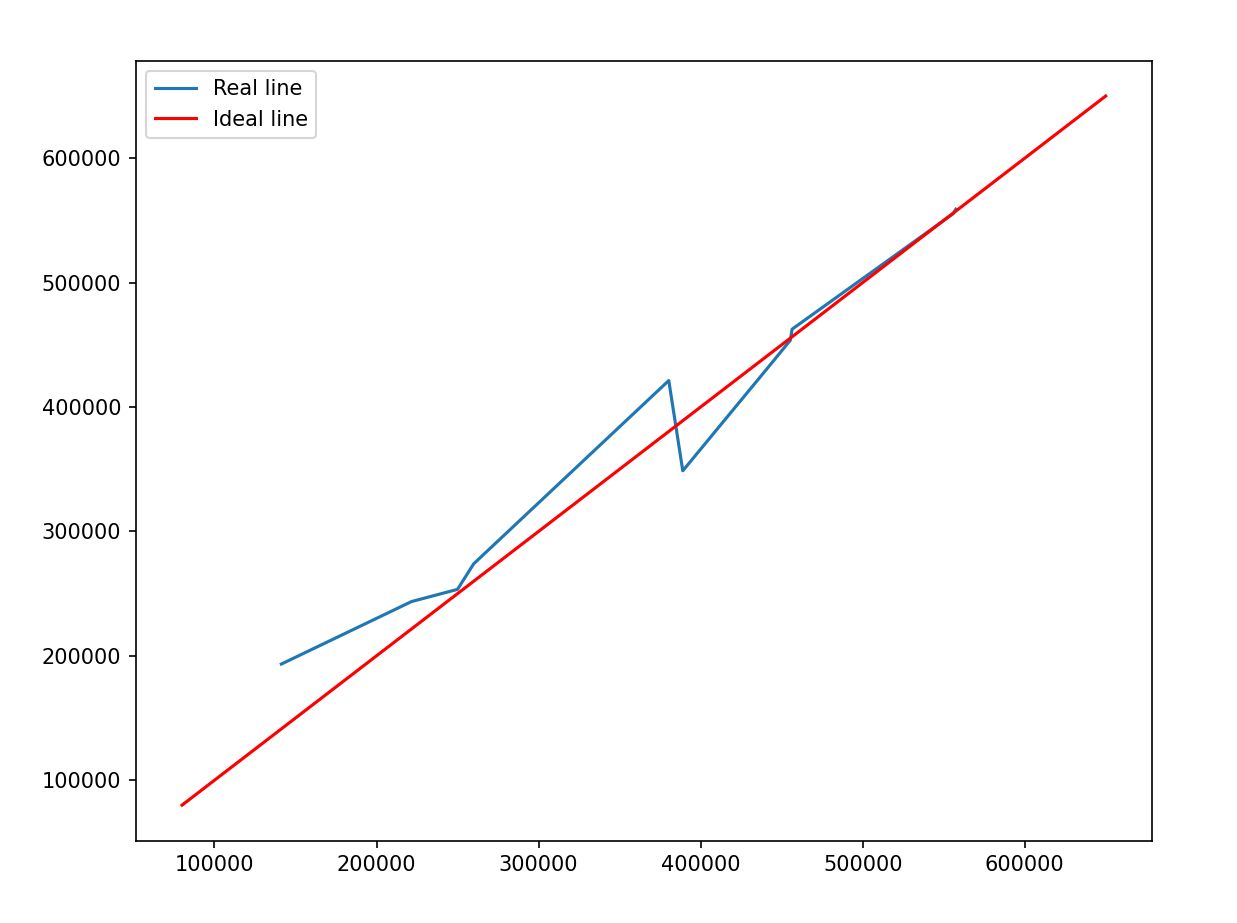
\includegraphics[width=\textwidth]{HK1.png}
    \caption{Monohulled Sailboats}\label{subfig:HK1}
    \end{subfigure}
    \begin{subfigure}[b]{.4\textwidth}
    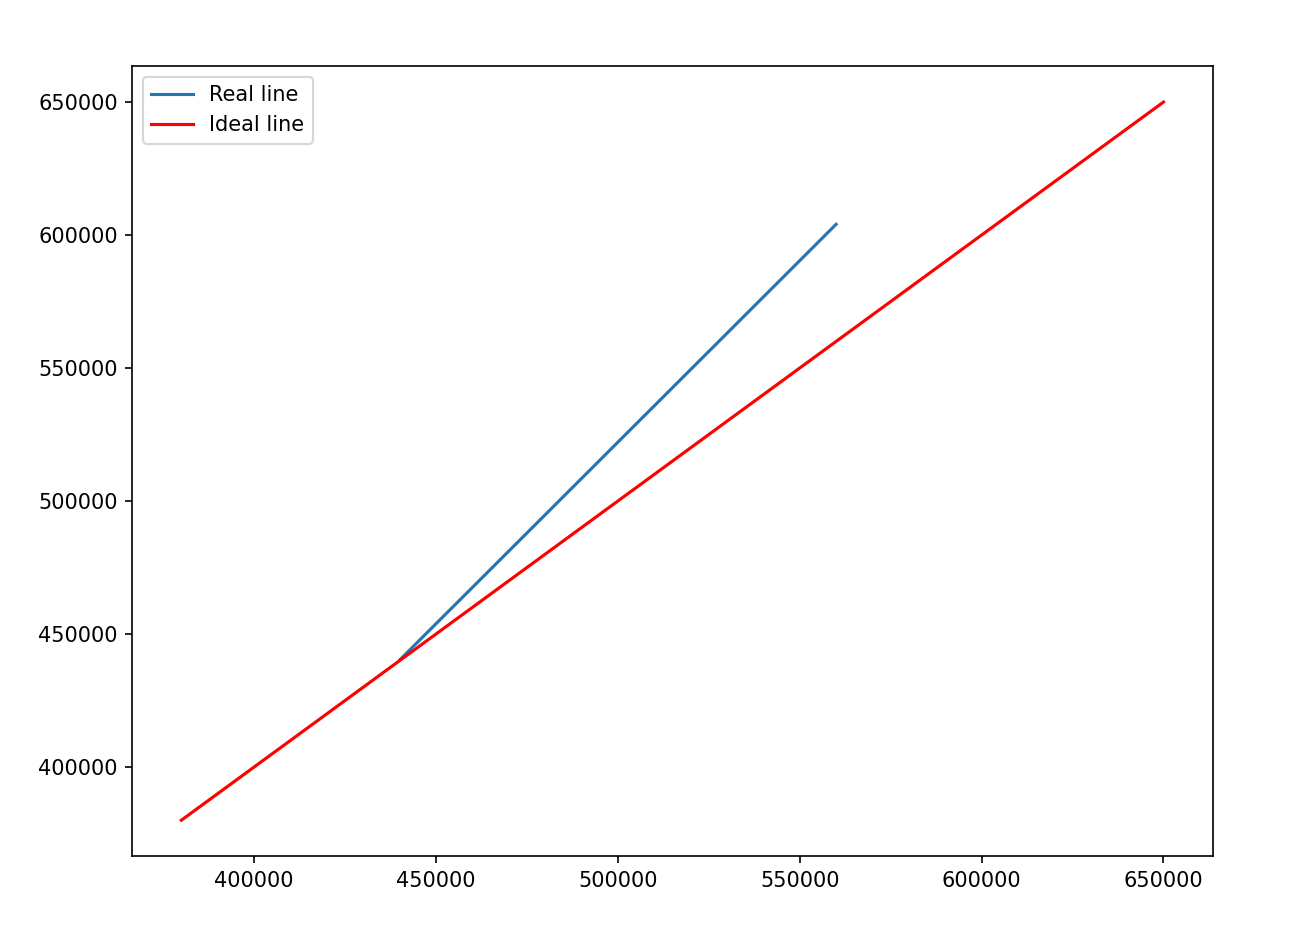
\includegraphics[width=\textwidth]{HK2.png}
    \caption{Catamaran}\label{subfig:HK2}
    \end{subfigure}
    \caption{Model Fitting Accuracy in HongKong}\label{fig:HK}
\end{figure} 

Interestingly, this regional effect is not observed in the subset of the monohulled sailboats market, suggesting that there are unique factors at play when it comes to the catamarans' market in Hong Kong. Upon further examination, we have deduced that the reason behind this discrepancy is likely due to Hong Kong's flourishing tourism industry.

Catamarans are widely regarded as superior to monohulled sailboats for travelers, offering a more stable and comfortable platform for sightseeing, relaxation, and entertainment. With the increasing number of tourists visiting Hong Kong, it is no surprise that the demand for catamarans has surged, thus contributing to the underestimation of our model's effectiveness in this particular market segment.

In conclusion, while our model has shown promising results in various aspects of the Hong Kong market, it is essential to recognize the unique regional factors that may affect its performance in certain subsets. By refining our model to account for these factors, we can ensure a more accurate and robust representation of the market dynamics at play. In doing so, our model will be better equipped to guide businesses and investors in making informed decisions, ultimately leading to a more prosperous and thriving economy in Hong Kong.


\section{Extended Inferences or Conclusion}
Upon conducting a thorough analysis of the relationship between various variables, excluding the average price and region, using linear correlation analysis tools, we have uncovered some intriguing patterns between the boat length and the region.

The analysis results reveal that people in European regions tend to prefer sailing longer boats, while individuals in the Caribbean area are fond of navigating more extended catamarans.

\section{Strengths and Weaknesses}
\subsection{Strengths}

\textbf{Strength-1 Comprehensiveness:}
After the basic data processing, we significantly expanded the dataset, including extending the Variant to Draft, Beam, Displacement, Water tank, Fuel tank, and Cabin, as well as expanding the Region to GDP per capita. We performed correlation tests for each variable, making the modeling process extensive and comprehensive.

\textbf{Strength-2 Innovative:}
Our model combines heuristic learning and hierarchical multivariate regression, obtaining accurate predictions through continuous iteration. This creative and highly applicable model is well-suited for the task at hand.Additionally, we used a deep forest algorithm to extend the prediction of unknown variants and regions, enhancing the model's versatility. 

\textbf{Strength-3 Accuracy:}
Our model performs exceptionally well in terms of both error analysis and accuracy, achieving 94.91\% on the Catamarans test set and 92.71\% on the Monohulled Boats test set. Moreover, the model can improve its accuracy through self-iteration and possesses heuristic learning capabilities.

\begin{figure}[htbp]
    \centering
    \begin{subfigure}[b]{.4\textwidth}
    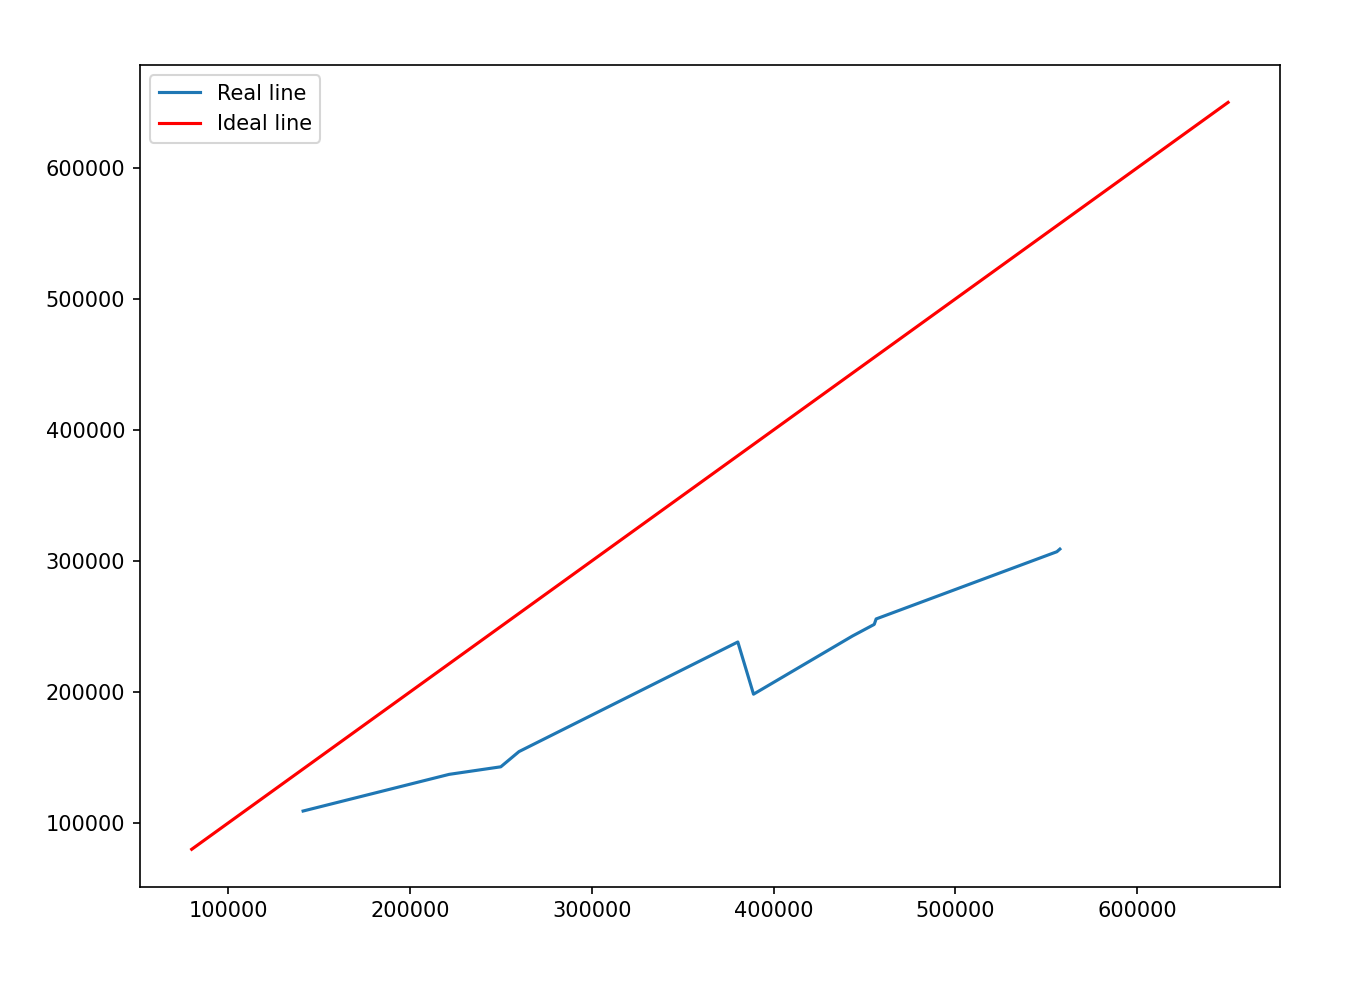
\includegraphics[width=\textwidth]{strength1.png}
    \caption{Single Cycle}\label{subfig:SG1}
    \end{subfigure}
    \begin{subfigure}[b]{.4\textwidth}
    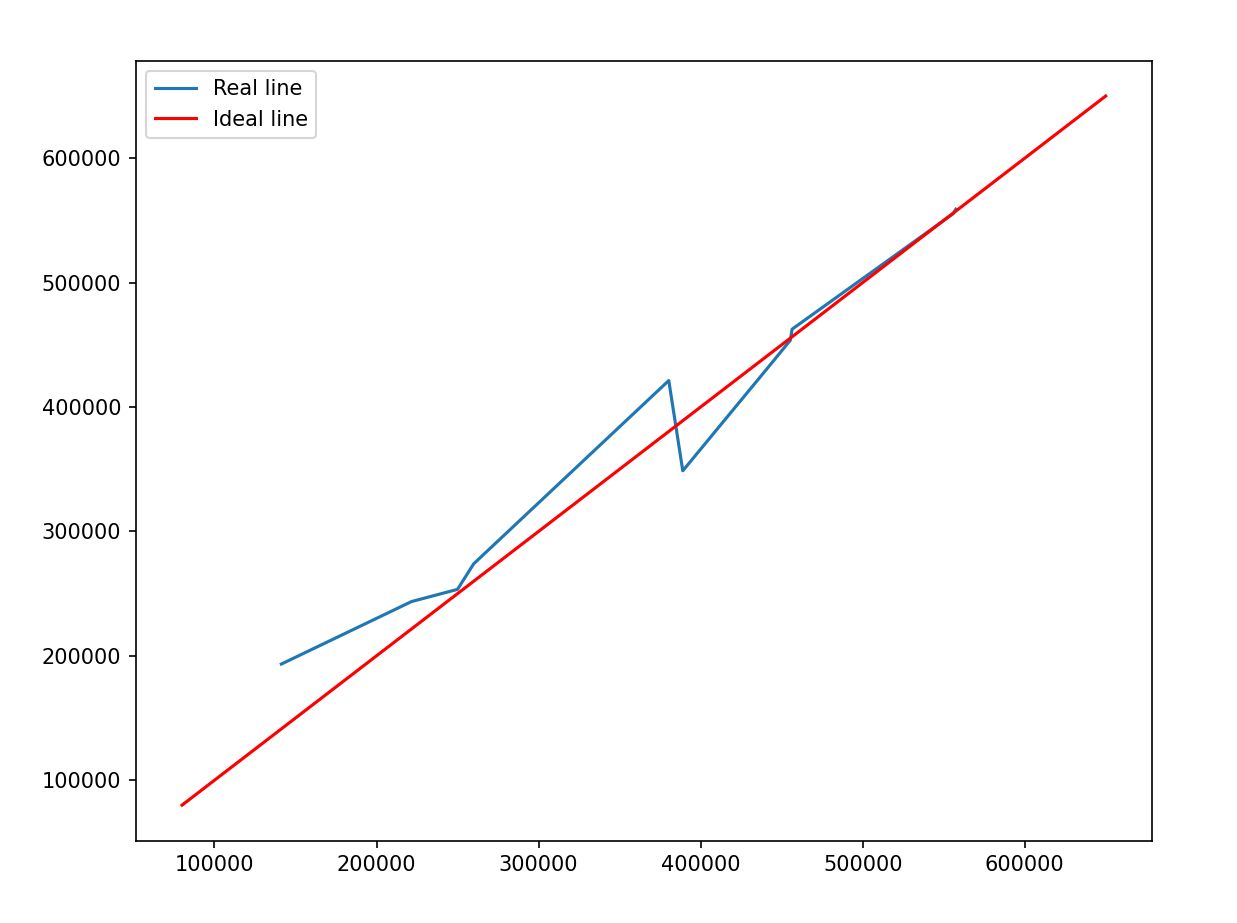
\includegraphics[width=\textwidth]{strength2.png}
    \caption{Muticycle}\label{subfig:SG2}
    \end{subfigure}
    \caption{Model accuracy improvement}\label{fig:strength}
\end{figure} 

\textbf{Strength-4 Applicability:}
When applied to the Hong Kong market, the model maintains a high level of accuracy, demonstrating its excellent applicability. 

\subsection{Weaknesses}
\textbf{Weakness-1 Time consuming:}
The model can achieve satisfactory regression results after 2-3 iterations when processing the data for this task. However, when handling larger datasets, the increased number of iterations may result in additional time costs.

\textbf{Weakness-2 Lack of geography  factor analysis:}
Due to the difficulty in obtaining geographical data and the challenge of analyzing and quantifying factors such as climate, the model does not include geographical factors. Despite this limitation, the model still provides valuable insights and accurate predictions for the used sailboat market.

\section{Further Improvements}
Although our Model has been optimized over several days, evolving from a simple decision tree to an organic combination of Heuristic Hierarchical Multiple Regression and Deep Forest, both \emph{Model 1} and \emph{Model 2} have produced excellent results in price prediction. However, during each iteration, we still only used a simple regression model, with accuracy being the result of iteration and heuristic learning. Upon reviewing the model, we identified the following two issues:
\begin{itemize}
    \item When fitting the Variant's Effect, we lost regional information.
    \item Combined Make and Variant, causing the model to overlook the premium issue between different Makes.
\end{itemize}
\subsection{Lasso Regression Update for Model}
To address the first issue, we decided to use Lasso Regression to replace the simple linear regression in each iteration process. The characteristics of Lasso Regression, which can avoid the problem of multicollinearity, also resolved the shortcomings of the original model. In each round of iterative regression, we only need to perform Lasso Regression on Variant and Region once, avoiding the loss of regional information. The specific formula is as follows:

$L_1,L_2$ regularization:
$$L_1=\lambda\sum_{j=1}^{p}|\beta_j|,L_2=\sum_{j=1}^{p}\beta_j^2$$

Lasso Regression's loss function:
$$\text{minizize }\frac{1}{2n}||y-X\beta||_2^2+\lambda||\beta||_1$$

Assume $\beta_i=\{\beta_{i1},\beta_{i2},\beta_{i3}\}$After introducing Lasso Regression, the model's process becomes:
\begin{itemize}
    \item \textbf{Step 1:} Since the relationship between year and price is highly linear, we first normalize the Year parameter to remove its influence,we can get $\beta_{11}$.
    \item \textbf{Step 2:} Then apply Lasso Regression to simultaneously normalize Variant and Region, combining the original functions $f_1(\beta_{12})\&g(\beta_{13})$ into $h_1(\beta_{12},\beta_{13})$.
    \item \textbf{Step 3:} Feeding $\beta_1=\{\beta_{11},\beta_{12},\beta_{13}\}$ into the iterative heuristic learning function. We perform iterative regression to obtain $h_1(\beta_{12},\beta_{13}),h_2(\beta_{22},\beta_{23}),\cdots,h_n(\beta_{n2},\beta_{n3})$ until the desired accuracy is reached, resulting in the final matrix $\beta_n=\{\beta_{n1},\beta_{n2},\beta_{n3}\}$.
    \item \textbf{Step 4:} Using $\beta_n$ for regression prediction, we obtain the predicted value.
\end{itemize}

This process is similar to the basic model idea. We also tried to update the model using Lasso Regression and re-predict the price. However, due to the lack of precision in the design matrix and the difficulty in controlling the regularization strength, the update was unsuccessful. Nonetheless, based on the initial improved model results and the Lasso Regression loss function, we can predict that the improved model will address multicollinearity issues for correlated Variant and Region variables.

\subsection{Better utilization of the Deep Forest}
As previously mentioned, we used Lasso Regression to address the issue of losing regional information when fitting the Variant's Effect. For the second issue, we considered fully utilizing Deep Forest by applying it to the regression process of \emph{Model 1}. Since Random Forest employs random sampling and feature selection, it can reduce the influence between correlated variables, thereby reducing multicollinearity problems, enhancing the stability and predictive accuracy of the regression model. Therefore, we do not need to combine Make and Variant into a single Variant variable for regression analysis. Instead, we can input all the screened variables into Deep Forest, allowing the model to self-prune and fit, enhancing robustness and generalization capabilities,then we get the graph below:

\begin{figure}[htbp]
    \centering
    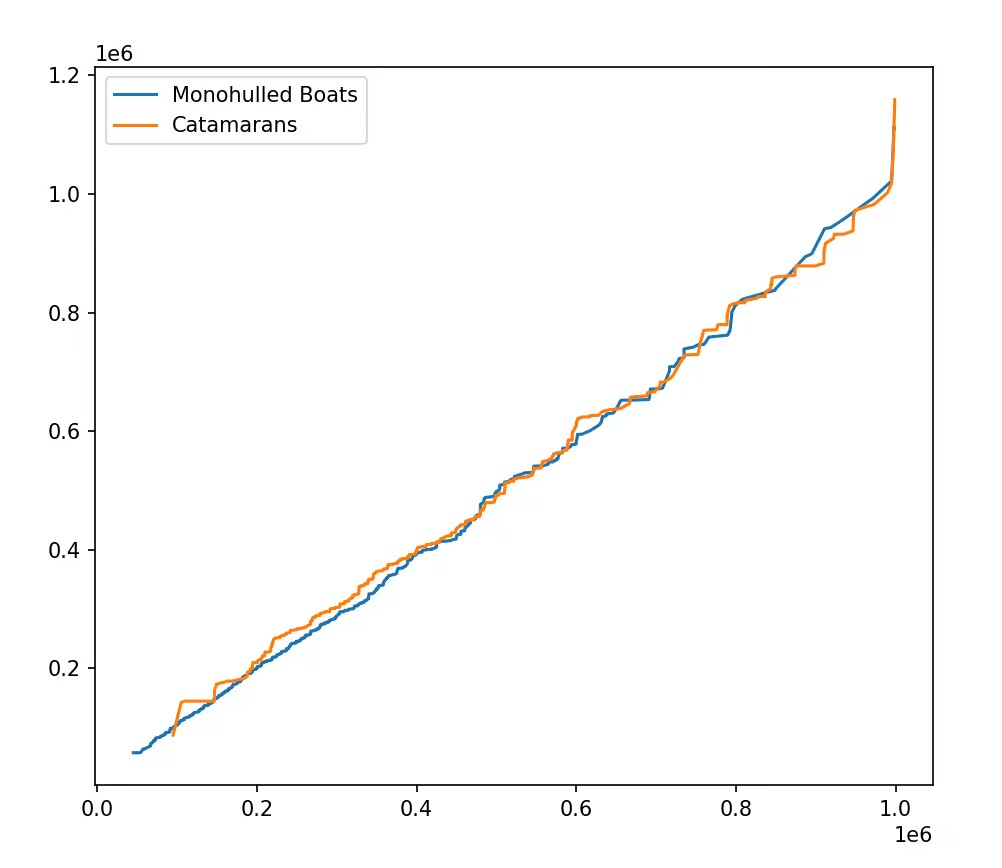
\includegraphics[width=.7\textwidth]{update.png}
    \caption{Optimizing Model Performance}\label{fig:update}
\end{figure}

We tested the optimized model on the training set and obtained the following results: Clearly, Deep Forest performs better in handling noise. However, on the other hand, due to the small dataset and the limited number of samples for some categories, Deep Forest exhibited some overfitting and underfitting phenomena. Moreover, since \emph{Model 2} also employed the Random Forest algorithm, this led to nested Random Forests, resulting in significant computational overhead. Compared to the increase in accuracy, the exponential growth of overhead is not worth the cost. Therefore, simply replacing the model with Deep Forest is not a perfect solution, and the model still requires further optimization and adjustment.However, from the preliminary results, it can be seen that the use of Deep Forest in the regression part does provide a solution to the second issue. We firmly believe that through structural adjustments, the model's performance will undoubtedly be further optimized!


\section{Conclusion}
In conclusion, our study has successfully addressed the challenges faced by brokers in the used sailboat market, where pricing is influenced by a myriad of factors such as brand, variant, age, depreciation rates, local consumption levels, and geographical environments. By developing a comprehensive and robust model that combines Heuristic Hierarchical Multiple Regression and Deep Forest Models, we have created a valuable tool that allows brokers and other stakeholders in the sailboat market to make well-informed decisions and ensure fair pricing practices.

Our meticulous data cleaning, expansion, and pre-analysis processes enabled us to establish a strong foundation for subsequent modeling efforts. Through Adaptive Density-Based Clustering and Linear interpolation techniques, we were able to identify patterns and trends in the data, providing crucial insights for our modeling approach.

The Heuristic Hierarchical Multiple Regression Model allowed us to establish the relationships between sailboat prices and factors such as year, region, and variant. Moreover, it enabled us to abstract the effect of regions and variants on sailboat prices, capturing the interactions between these variables and their influence on pricing.

By employing the Deep Forest Model, we trained the relationship between region and variant factors and their respective effects. This advanced ensemble learning technique enabled us to predict the effect of unknown regions and variants, which in turn allowed us to further predict their prices.

Our model has proven to be highly effective, achieving remarkable accuracy levels of 94.91\% on the Catamarans test set and 92.71\% on the Monohulled Boats test set. These results demonstrate the model's strong performance and applicability to real-world scenarios. Furthermore, the model's self-iteration and heuristic learning capabilities ensure that it can continuously improve its accuracy, making it an invaluable tool for brokers in the used sailboat market.

When applied to the Hong Kong market, our model maintained a high level of accuracy, showcasing its excellent applicability across different regions. The model's ability to achieve satisfactory regression results after 2-3 iterations is particularly noteworthy, as it demonstrates its efficiency and effectiveness in handling diverse datasets.

While our model does not currently include geographical factors due to the challenges in obtaining and quantifying geographical data, future research could explore incorporating these factors to further enhance the model's predictive capabilities.

In summary, our study has successfully developed a powerful and versatile model that can assist brokers in the used sailboat market in making more reasonable and comprehensive evaluations, ultimately leading to more rational and fair pricing practices. By combining the strengths of Heuristic Hierarchical Multiple Regression and Deep Forest Models, we have created a valuable tool that can be applied to various markets and datasets, making it an invaluable asset for brokers and stakeholders in the used sailboat market.
% 以下为信件/备忘录部分,不需要可自行去掉
% 如有需要可将整个 letter 环境移动到文章开头或中间
% 请在第二个花括号内填写标题,如「信件」(Letter)或「备忘录」(Memorandum)
\begin{letter}{Report}
\noindent\rule[0.25\baselineskip]{\textwidth}{2pt} 
\begin{flushleft}  % 左对齐环境,无首行缩进
\textbf{To:} The sailboat broker in Hong Kong\\
\textbf{From:} Team \#2332102\\
\textbf{Date:} Apr 3th, 2023\\
\textbf{Subject:} 
\noindent\rule[0.25\baselineskip]{\textwidth}{1pt}
\end{flushleft}

\noindent \textbf{\emph{Part One - Model Accuracy}}

\begin{figure}[htbp]
    \centering
    \begin{subfigure}[b]{.4\textwidth}
    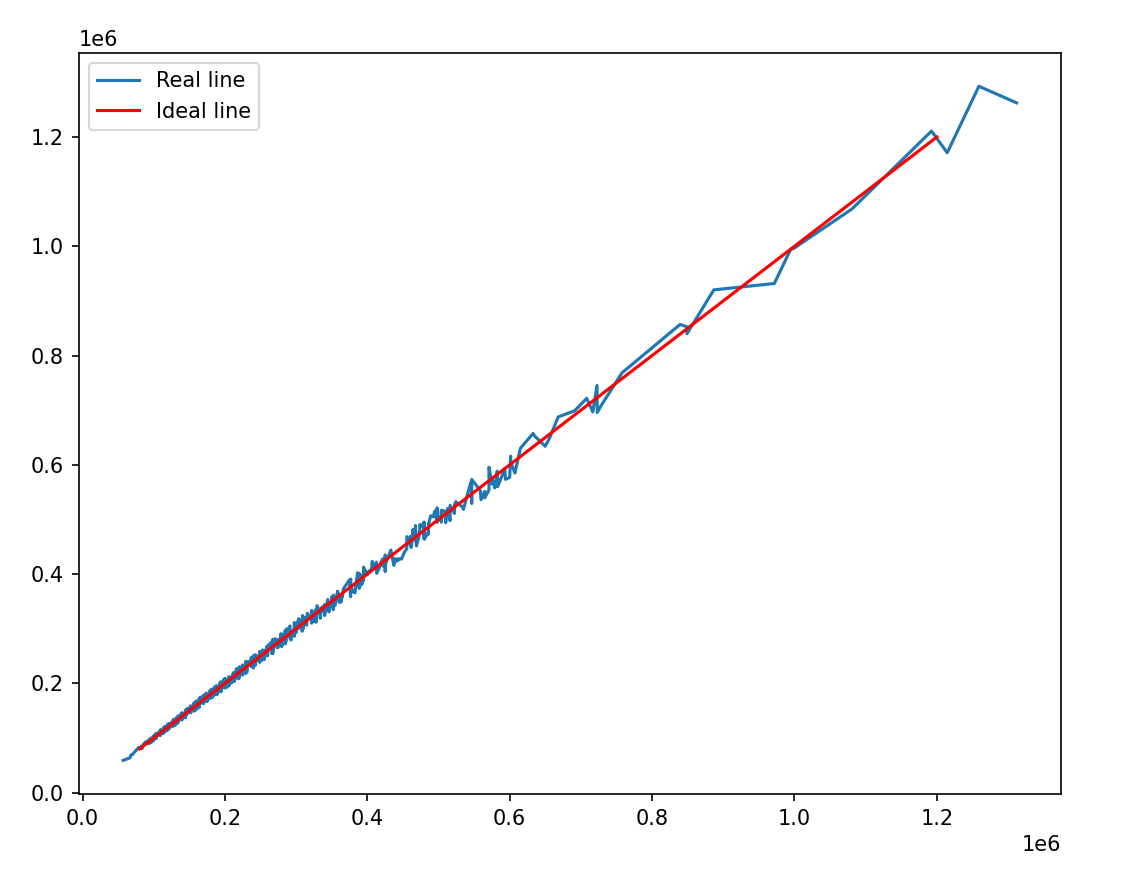
\includegraphics[width=\textwidth]{report1.png}
    \caption{Monohulled Sailboats}\label{subfig:report1}
    \end{subfigure}
    \begin{subfigure}[b]{.4\textwidth}
    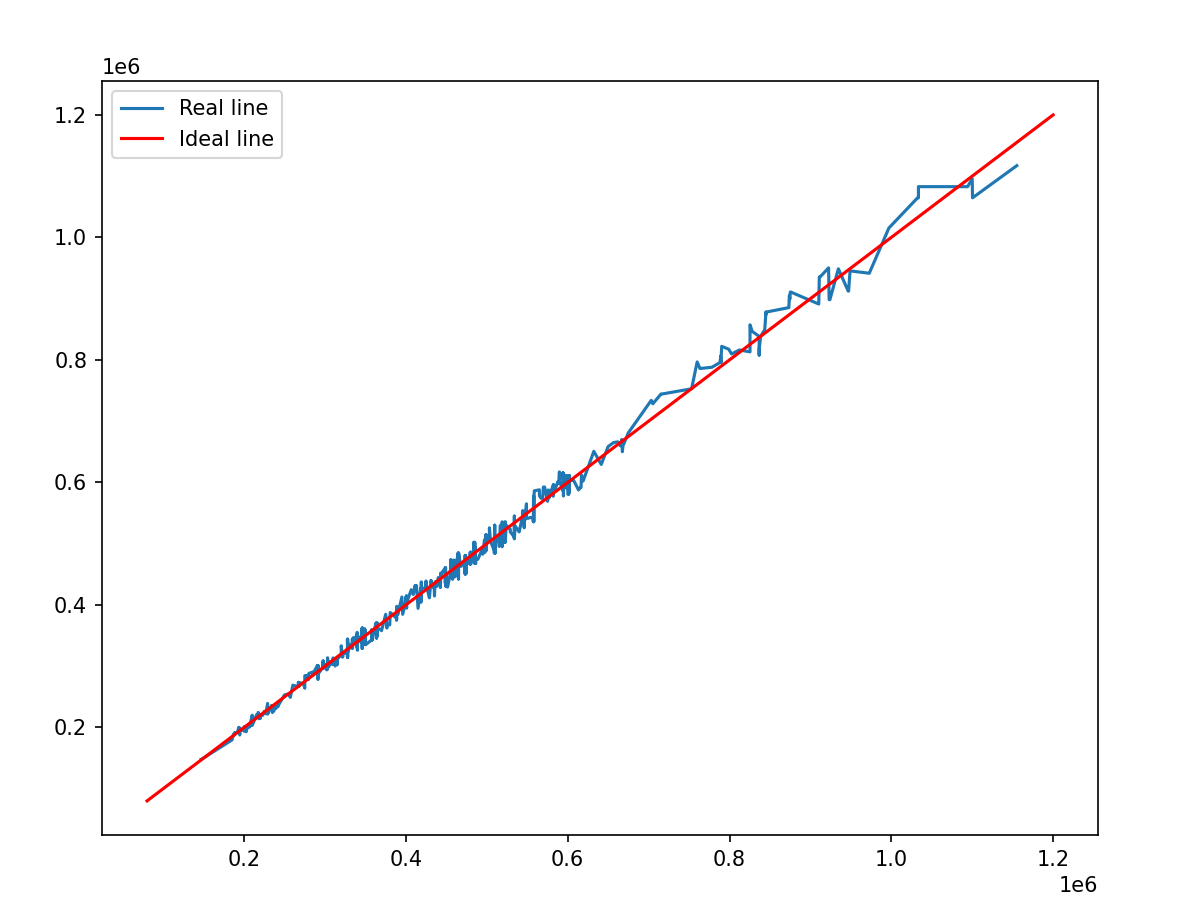
\includegraphics[width=\textwidth]{report2.png}
    \caption{Catamaran}\label{subfig:report2}
    \end{subfigure}
    \caption{Model Fitting Accuracy}\label{fig:Report1}
\end{figure} 

The two line charts presented above use the actual prices as the x-axis and the predicted values from our model as the y-axis. The fit between the line and the $y=x$ equation demonstrates the accuracy of our model. Clearly, our model is highly effective in predicting the prices of used boats worldwide. We have tested the model's accuracy, achieving 94.91\% for Catamarans and 92.61\% for Monohulled Sailboats. Thus, our model is fundamentally accurate in its price predictions.

\noindent \textbf{\emph{Part Two - Analysis of Variance}}

\begin{figure}[htbp]
    \centering
    \begin{subfigure}[b]{.4\textwidth}
    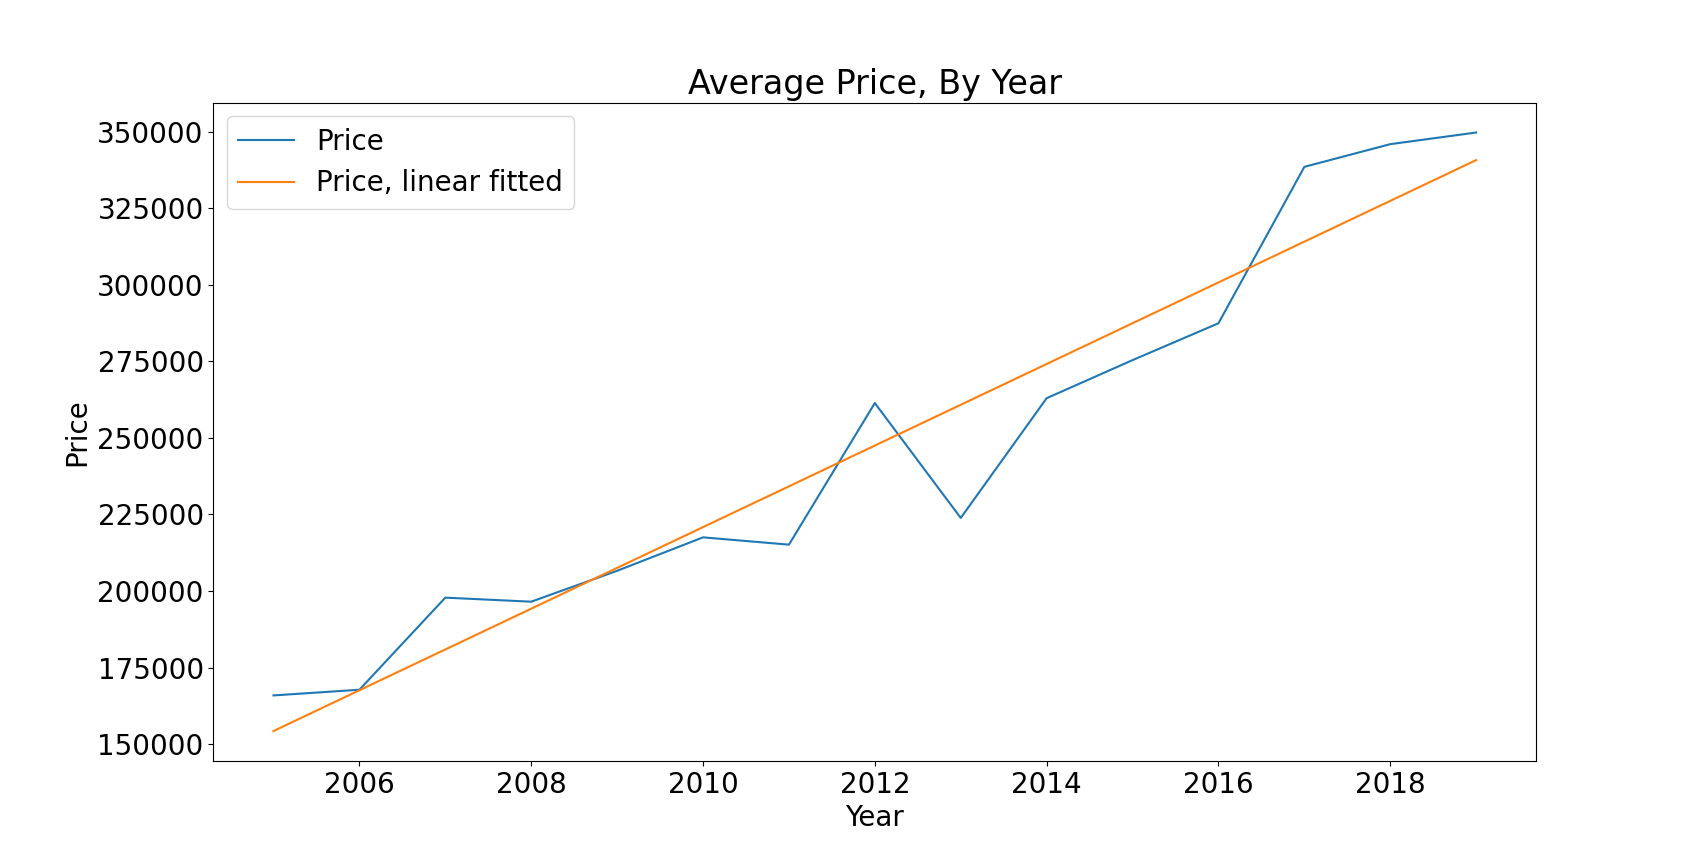
\includegraphics[width=\textwidth]{monohulled_price_year.png}
    \caption{Monohulled Sailboats}\label{subfig:report3}
    \end{subfigure}
    \begin{subfigure}[b]{.4\textwidth}
    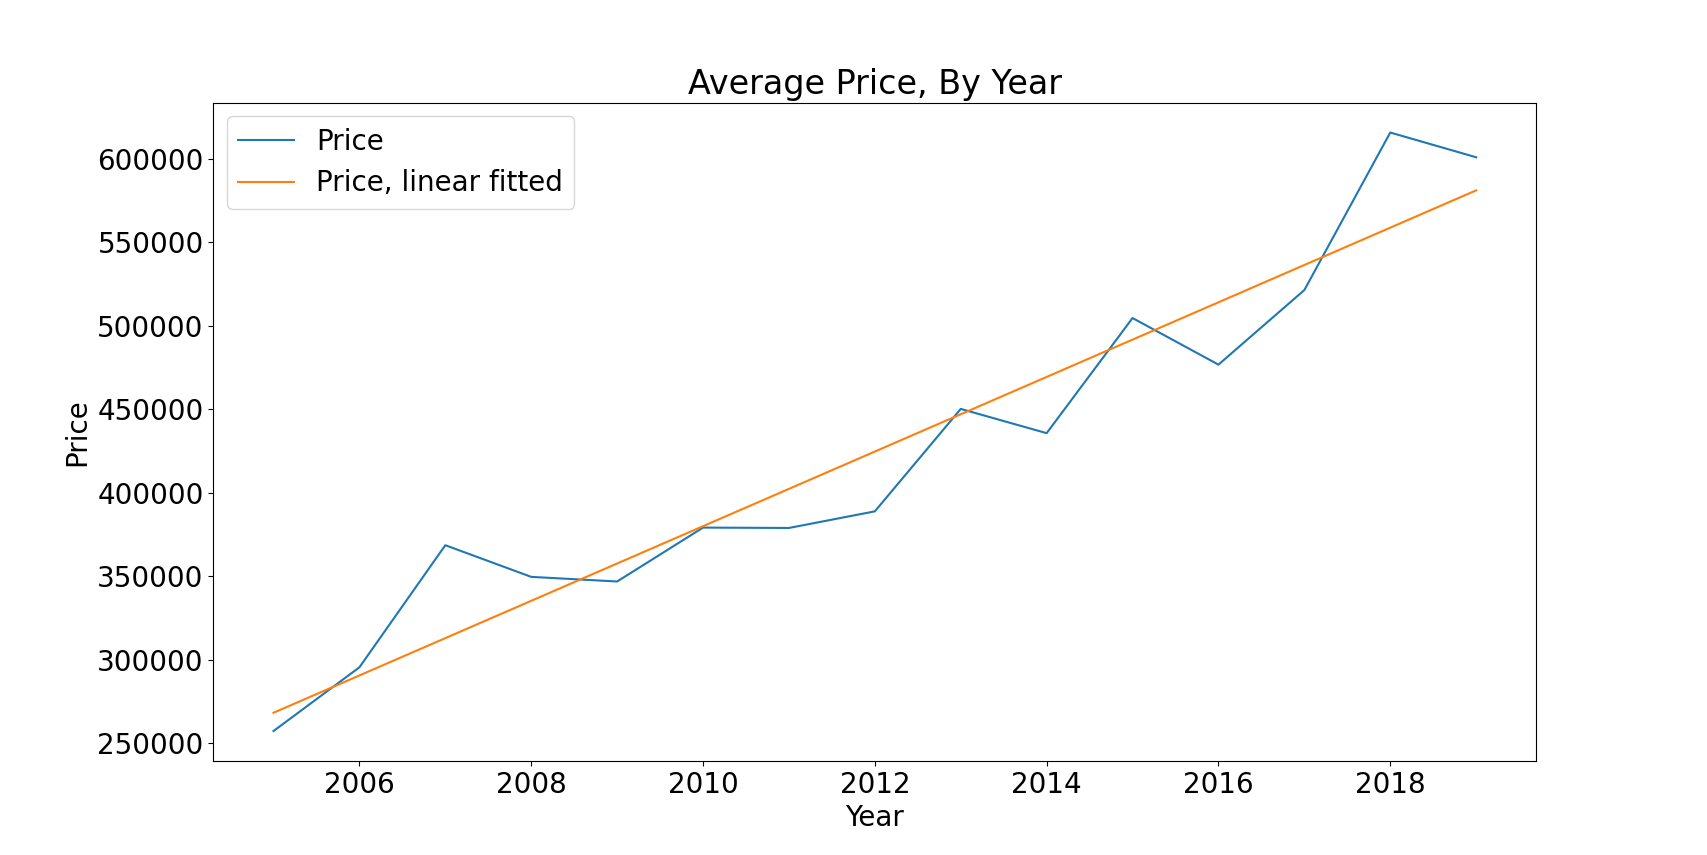
\includegraphics[width=\textwidth]{catamaran_price_year.png}
    \caption{Catamaran}\label{subfig:report4}
    \end{subfigure}
    \caption{The relationship between year and price}\label{fig:Report2}
\end{figure} 

Figure 15 reveals a strong linear correlation between price and year. The model shows that the Region's Effect influences market prices by affecting boat types. In particular, areas with higher per capita GDP tend to buy more expensive boat types, leading to higher average prices for used boats in these regions.
\clearpage
\noindent \textbf{\emph{Part Three - Model of Hong Kong}}

\begin{figure}[htbp]
    \centering
    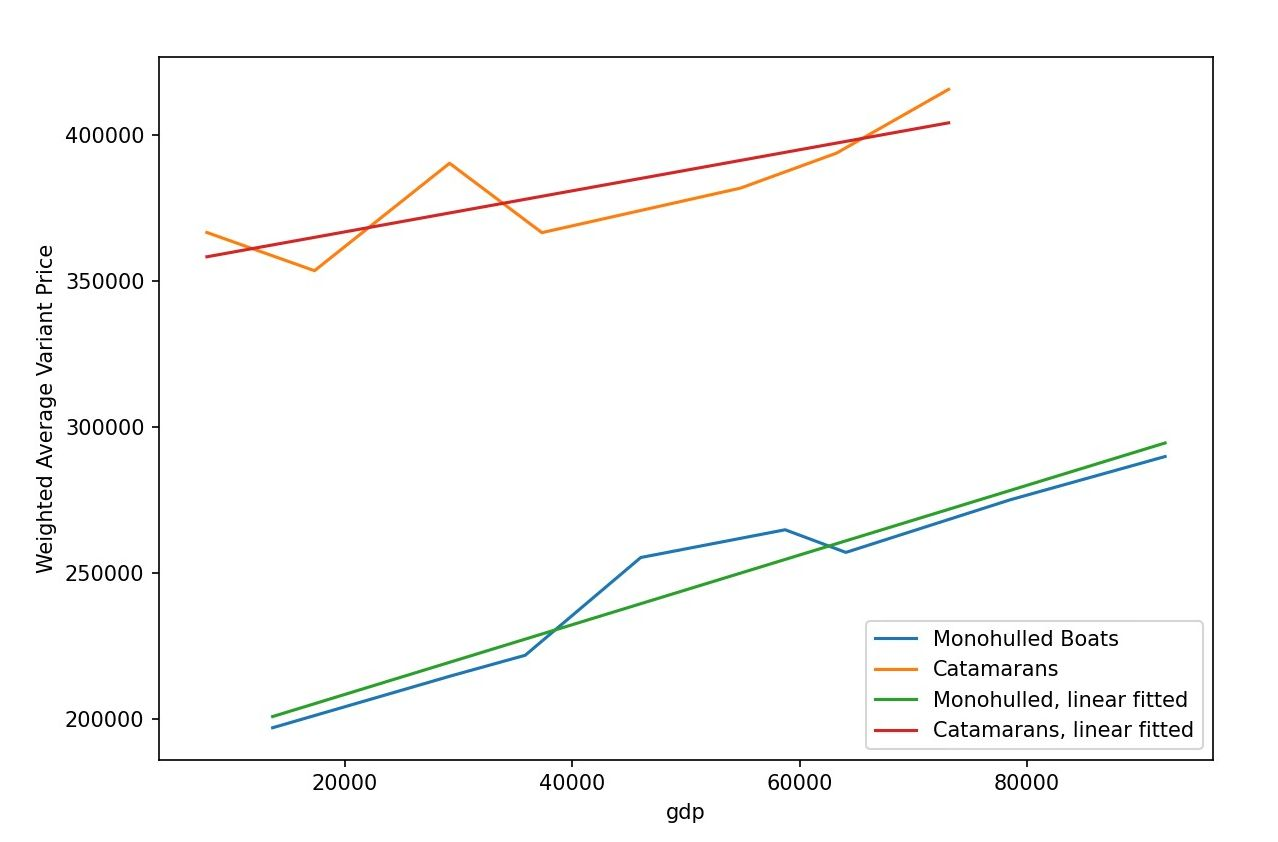
\includegraphics[width=.5\textwidth]{report5.jpg}
    \caption{Optimizing Model Performance}\label{fig:Report3}
\end{figure}

Comparing the slopes of the two regression models in Figure 4, we see that regional economic conditions impact both boat types. However, in Hong Kong, we found that the extra-regional effect is not found in the subset of the monohulled sailboats market. We infer that this is probably because of Hong Kong's prosperous tourism -- catamarans are better than monohulled sailboats for travelers.

\noindent \textbf{\emph{Part Four - Interesting Conclusion}}

\begin{figure}[htbp]
    \centering
    \begin{subfigure}[b]{.45\textwidth}
    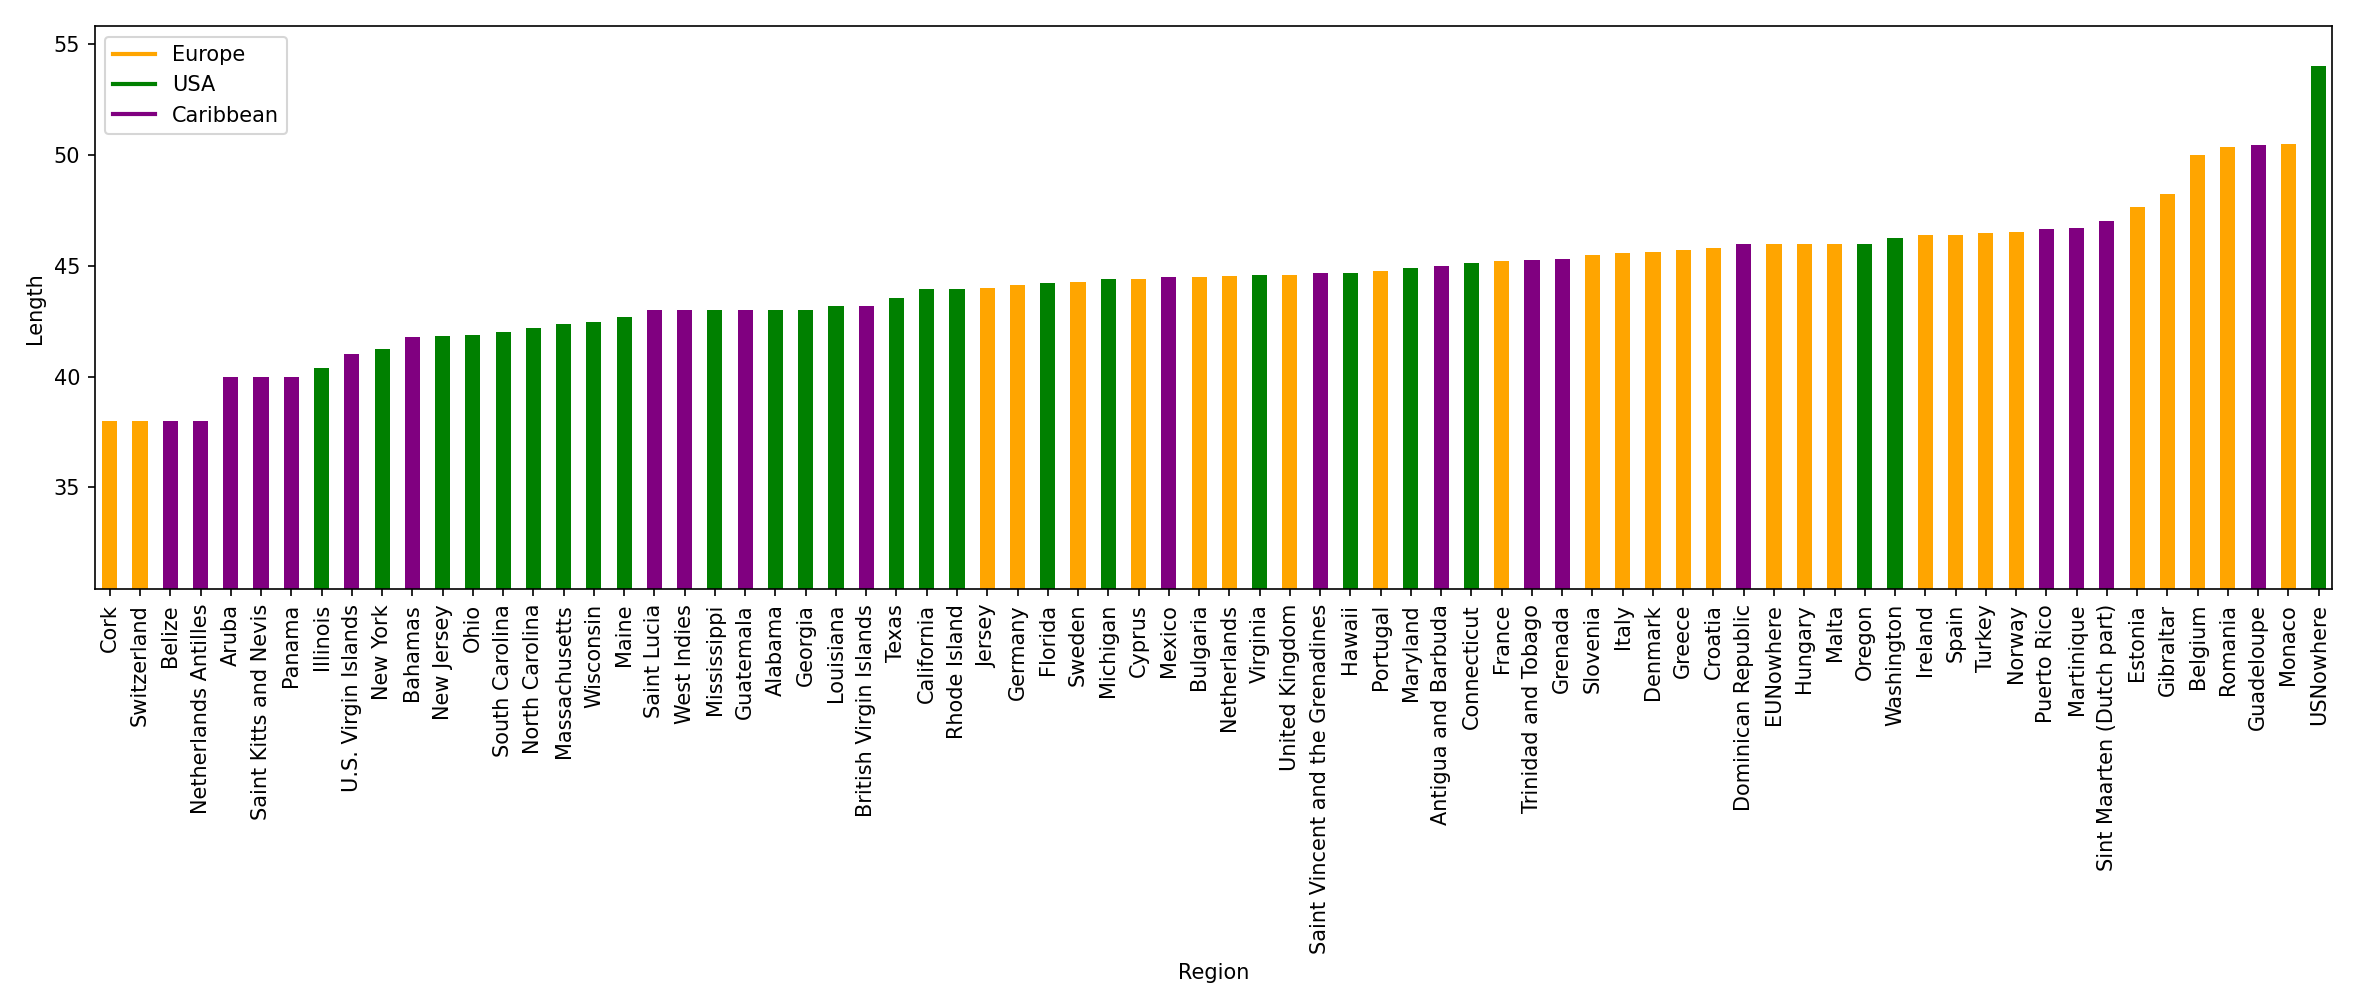
\includegraphics[width=\textwidth]{report3.png}
    \caption{Monohulled Sailboats}\label{subfig:report5}
    \end{subfigure}
    \begin{subfigure}[b]{.4\textwidth}
    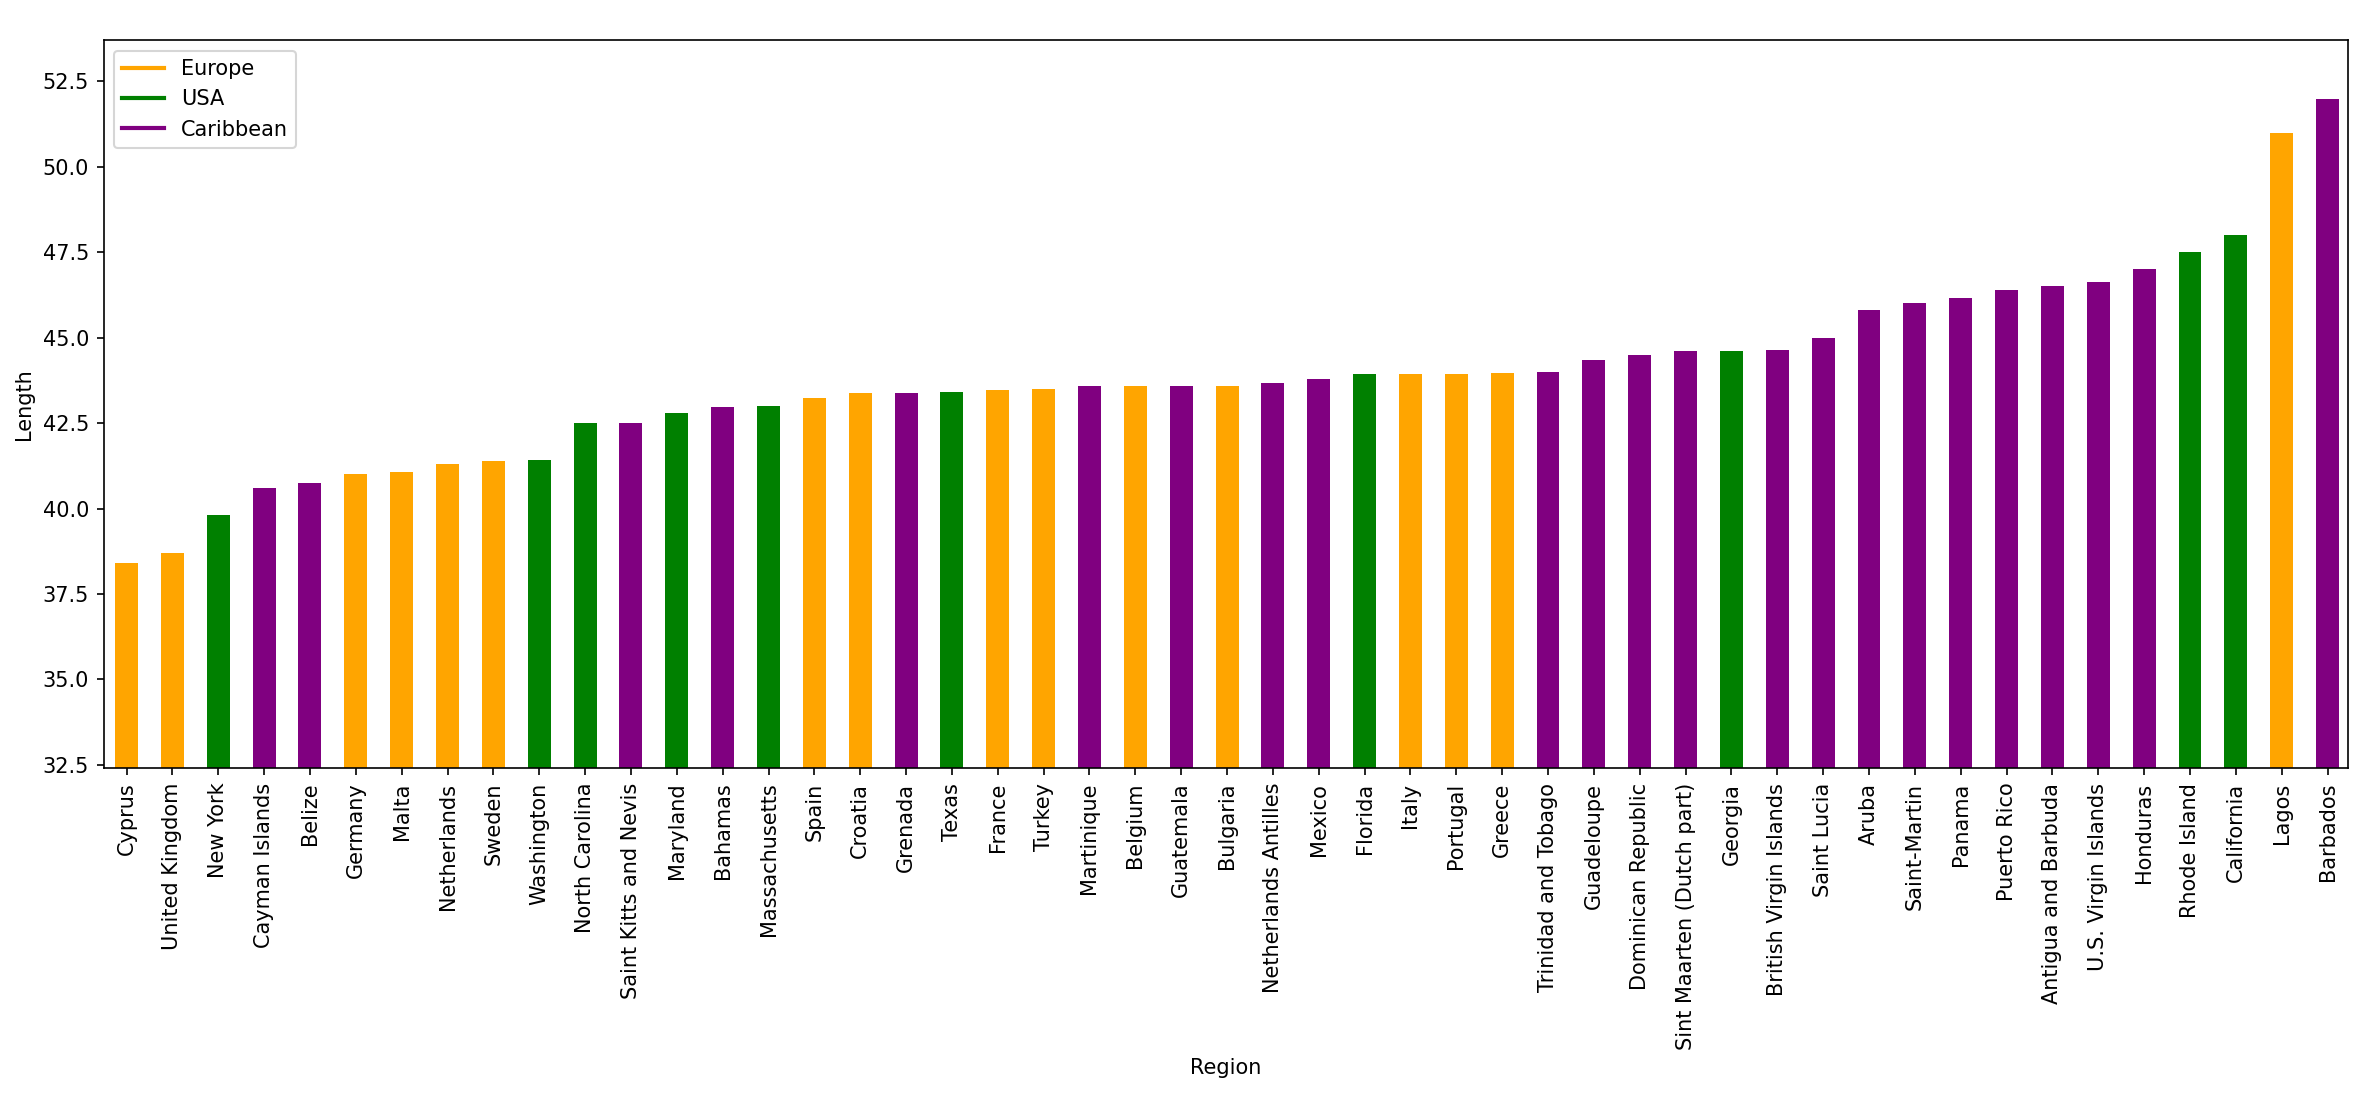
\includegraphics[width=\textwidth]{report4.png}
    \caption{Catamaran}\label{subfig:report6}
    \end{subfigure}
    \caption{Preferences for boat lengths vary among different regions}\label{fig:Report4}
\end{figure} 

Based on the two bar charts, we have drawn an interesting conclusion: the analysis results reveal that people in European regions tend to prefer sailing longer boats, while individuals in the Caribbean area are fond of navigating more extended catamarans. This phenomenon may be related to local geography and culture.

\noindent\rule[0.25\baselineskip]{\textwidth}{2pt} 
\end{letter}

\clearpage

% 参考文献,此处以 MLA 引用格式为例
\begin{thebibliography}{99}
\bibitem{1} Zhi-Hua Zhou, Ji Feng, Deep forest, \emph{National Science Review}, January 2019, from\url{https://doi.org/10.1093/nsr/nwy108}.
\bibitem{2} Eberly, L.E. (2007). Multiple Linear Regression. \emph{Methods in Molecular Biology}, from \url{https://doi.org/10.1007/978-1-59745-530-5_9}.
\bibitem{3} A. Ogunleye and Q. -G. Wang, "XGBoost Model for Chronic Kidney Disease Diagnosis," in \emph{IEEE/ACM Transactions on Computational Biology and Bioinformatics}.
\bibitem{4} Ingo Steinwart. "Fully adaptive density-based clustering." Ann. Statist, from \url{https://doi.org/10.1214/15-AOS1331}.
\bibitem{5} Reiss, K., Renkl, A. Learning to prove: The idea of heuristic examples. \emph{Zentralblatt für Didaktik der Mathematik}, from \url{https://doi.org/10.1007/BF02655690}.
\bibitem{6} Larson M G. Analysis of variance[J]. Circulation.
\bibitem{7} Witten I H, Frank E, Hall M A, et al. Practical machine learning tools and techniques[C].
\bibitem{8} Myles A J, Feudale R N, Liu Y, et al. An introduction to decision tree modeling[J].
\bibitem{9} Biau G, Scornet E. A random forest guided tour[J].
\bibitem{10} Genesove D. Adverse selection in the wholesale used car market[J].
\bibitem{11} Bernard H R, Ryan G. Text analysis[J]. 
\bibitem{12} Davis P J. Interpolation and approximation[M]. Courier Corporation, 1975.
\bibitem{13} Ganaie M A, Hu M, Malik A K, et al. Ensemble deep learning: A review[J].
\bibitem{14} Zhang M L, Zhou Z H. ML-KNN: A lazy learning approach to multi-label learning[J].
\bibitem{15} Madhulatha T S. An overview on clustering methods[J].
\bibitem{16} Limsombunchao V. House price prediction, hedonic price model.
\end{thebibliography}

\end{document}  % 结束
